\documentclass[oneside,10pt]{memoir}

\usepackage{microtype}
\usepackage{mathptmx}
\usepackage{graphicx}
\usepackage{amsmath}
\usepackage{bigstrut}
\usepackage{hyperref}
\usepackage{xfrac}
\usepackage{siunitx}
\usepackage{fancyvrb}
\usepackage{pdfpages}

\settocdepth{subsection}
\headstyles{bringhurst}
\hypersetup{bookmarksopen,
            bookmarksnumbered,
            colorlinks=true,
            citecolor=red,
            filecolor=red,
            urlcolor=red}

\newsubfloat{figure}
\makepagenote

\sisetup{group-separator={,}}
%\sisetup{group-minimum-digits={4},group-separator={,}}

%-------------------------------------------------------------------------------

\newcommand{\twod}    {2D}
\newcommand{\threed}  {3D}
\newcommand{\opengl}  {\textsc{OpenGL}}
\newcommand{\scm}     {\textsc{scm}}
\newcommand{\tiff}    {\textsc{tiff}}
\newcommand{\bigtiff} {Big\textsc{tiff}}
\newcommand{\libtiff} {lib\textsc{tiff}}
\newcommand{\xml}     {\textsc{xml}}
\newcommand{\img}     {\textsc{img}}
\newcommand{\api}     {\textsc{api}}
\newcommand{\scmtiff} {\texttt{scmtiff}}
\newcommand{\scmview} {\texttt{scmview}}
\newcommand{\scmpath}{\texttt{SCMPATH}}
\newcommand{\rgb}     {\textsc{rgb}}
\newcommand{\mb}    {\,\textsc{mb}}
\newcommand{\vram}    {\textsc{vram}}
\newcommand{\panoview}{\textsc{PanoView}}
\newcommand{\orbiter} {\textsc{Orbiter}}

\newcommand{\B}{\bigstrut[b]}
\newcommand{\T}{\bigstrut[t]}
\newcommand{\X}[1]{\smash{#1}\phantom{o}}

\newcommand{\Pos}[1]{\phantom{-}{#1}}
\newcommand{\Neg}[1]{        {-}{#1}}

\newcommand{\inangles}[1]{$\langle$#1$\rangle$}

\newcommand{\scmcount} [1]{\ensuremath{\mathit{count}(#1)}}
\newcommand{\scmwidth} [1]{\ensuremath{\mathit{width}(#1)}}
\newcommand{\scmheight}[1]{\ensuremath{\mathit{height}(#1)}}
\newcommand{\scmlevel} [1]{\ensuremath{\mathit{level}(#1)}}
\newcommand{\scmroot}  [1]{\ensuremath{\mathit{root}(#1)}}
\newcommand{\scmrank}  [1]{\ensuremath{\mathit{rank}(#1)}}
\newcommand{\scmrow}   [1]{\ensuremath{\mathit{row}(#1)}}
\newcommand{\scmcol}   [1]{\ensuremath{\mathit{col}(#1)}}
\newcommand{\scmindex} [1]{\ensuremath{\mathit{index}(#1)}}
\newcommand{\scmparent}[1]{\ensuremath{\mathit{parent}(#1)}}
\newcommand{\scmchild} [1]{\ensuremath{\mathit{child}(#1)}}
\newcommand{\scmnorth} [1]{\ensuremath{\mathit{north}(#1)}}
\newcommand{\scmsouth} [1]{\ensuremath{\mathit{south}(#1)}}
\newcommand{\scmwest}  [1]{\ensuremath{\mathit{west}(#1)}}
\newcommand{\scmeast}  [1]{\ensuremath{\mathit{east}(#1)}}

\newenvironment{optionlist}
  {\setlength{\leftmargini}{1in}\begin{itemize}}{\end{itemize}}

\renewcommand{\descriptionlabel}[1]{\qquad\textit{#1}}

\RecustomVerbatimEnvironment{Verbatim}{Verbatim}{numbers=left,fontsize=\small}

%-------------------------------------------------------------------------------

\begin{document}
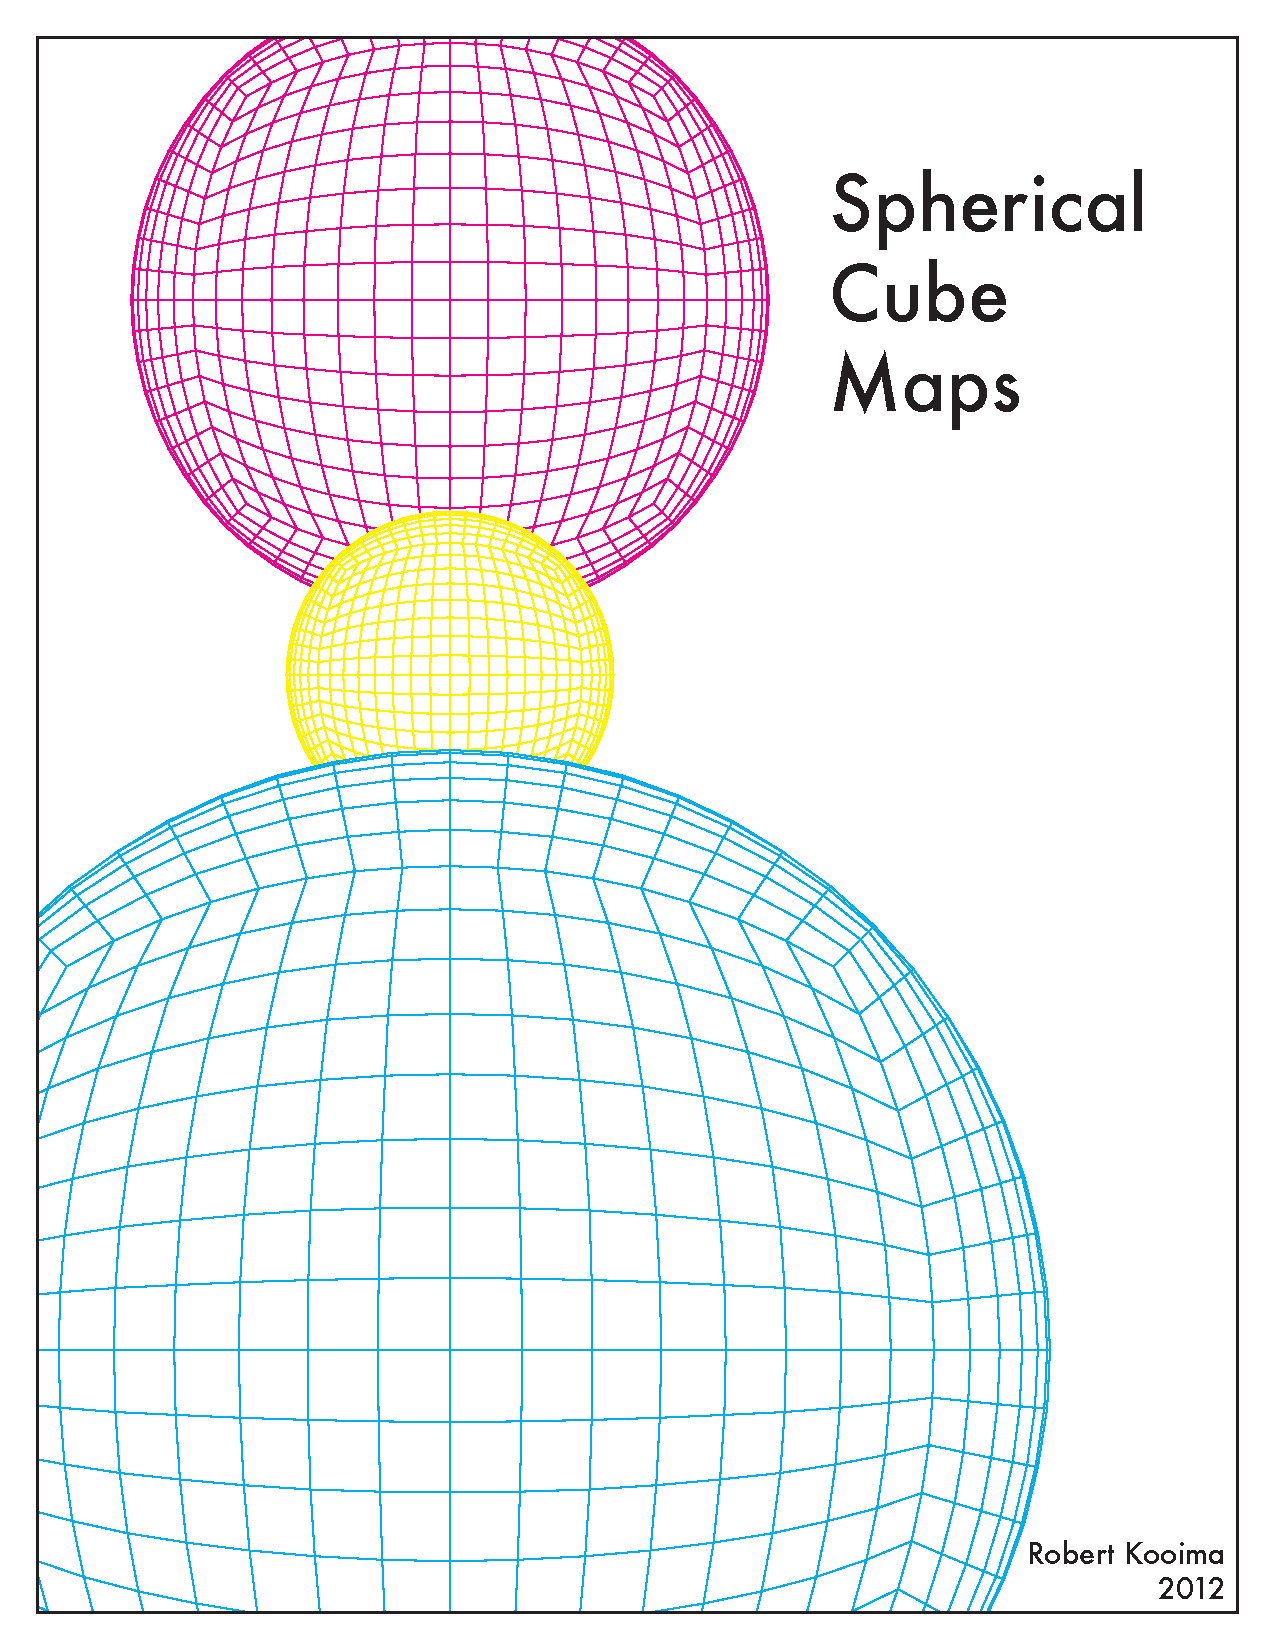
\includepdf{fig/titlepage.pdf}

\begin{Spacing}{1.1}

% SCMTIFF
%     Many modes

% Example: WAC global ortho blending
% Example: WAC DTM / LOLA merge

% Appendix: Panoview configuration

\tableofcontents

%------------------------------------------------------------------------------

\chapter{Spherical Cube Map}

\section{Spherical sampling}
\label{sec:sampling}

The mapping of image data onto the sphere is intuitively similar to a standard \opengl\ cube map. Begin by considering an $n\times n$ raster image applied to the $+Z$ face of a cube. For a spherical cube map, the pixel at row~$r$ and column~$c$ gives a sample at a position $(\alpha, \beta)$ on the sphere, where
\[\alpha=90^{\circ}\,\frac{c + \sfrac{1}{2}}{n} - 45^{\circ}\qquad\beta=90^{\circ}\,\frac{r + \sfrac{1}{2}}{n} - 45^{\circ}.\]
This corresponds to the \threed\ vector
\[v=\left[\begin{array}{c}
\phantom{-}\sin\alpha\, \cos\beta\\
        {-}\cos\alpha\, \sin\beta\\
\phantom{-}\cos\alpha\, \cos\beta
\end{array}\right].\]

This vector has length \(\sqrt{\cos^2\,\alpha + \sin^2\,\alpha\,\cos^2\,\beta}\), but when normalization is required, one will probably prefer the more familiar divisor \(\sqrt{v_x^2+v_y^2+v_z^2}\).

Vectors within the remaining cube faces are simple \ang{90} rotations of the definition for $+Z$, trivially implemented in the form of swizzles and negations. For each face, the vector $(x', y', z')$ is defined in terms of $(x, y, z)$ as follows.
\begin{center}
\begin{tabular}{rr|r|r|r|r|r}
    &$\Pos{X}$&$\Neg{X}$&$\Pos{Y}$&$\Neg{Y}$&$\Pos{Z}$&$\Neg{Z}$\B\\\hline
$x'=$&$\Pos{z}$&$\Neg{z}$&$\Pos{x}$&$\Pos{x}$&$\Pos{x}$&$\Neg{x}$\T\\
$y'=$&$\Pos{y}$&$\Pos{y}$&$\Pos{z}$&$\Neg{z}$&$\Pos{y}$&$\Pos{y}$\\
$z'=$&$\Neg{x}$&$\Pos{x}$&$\Neg{y}$&$\Pos{y}$&$\Pos{z}$&$\Neg{z}$\\
\end{tabular}
\end{center}

The cube face orientations given by this swizzle table match the definition of a standard \opengl\ linear cube map. It is the non-linear mapping from row and column to 3D vector that puts the ``spherical'' in ``spherical cube map.'' While more expensive to compute, this mapping is more amenable to the delivery of high resolution spherical data sets, as it provides a more uniform tesselation of the sphere, and thus a more consistent density of data at every point on its surface.

As depicted by Figure~\ref{fig:cube}, linear cube map samples stretch in the center of the face and compress toward the edges. While all tessellations of the sphere necessarily demonstrate some degree of similar non-uniformity, the spherical cube map, Figure~\ref{fig:scube}, is visibly closer to the impossible ideal. Specifically, the very smallest samples of a linear cube map, found at the corners, have only $19\%$ of the area of the largest samples at the cube face centers. That is, samples near the center of a cube map face cover more than \emph{five times} the area of samples at the corners. In contrast, the smallest samples of a spherical cube map face, found at the centers of the face edges, have $70\%$ of the area of the largest samples at the face centers.\pagenote{In an unexpected result, as the resolution of an \scm\ page tends toward infinity, the ratio of the solid angle of a center pixel (the largest pixel) to the solid angle of an edge pixel (the smallest pixel) tends toward exactly $\sqrt{2}/2$.} The corner samples of an \scm\ are actually \emph{not} the smallest, with $76\%$ the area of the center samples.

\begin{figure}
  \centering
  \subbottom[Linear cube map]{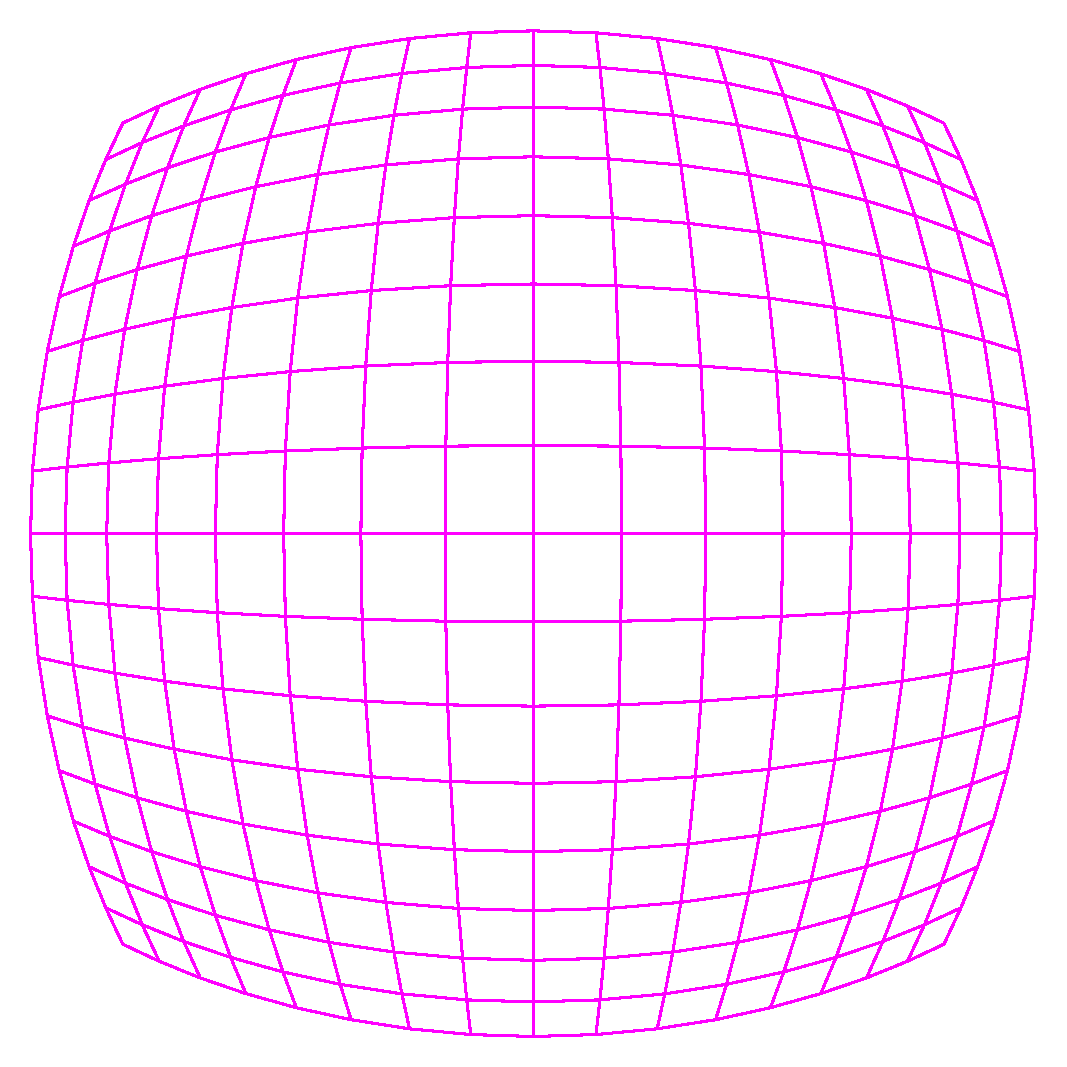
\includegraphics[width=0.3\textwidth]{fig/cube.pdf}\label{fig:cube}}
  \hfil
  \subbottom[Spherical cube map]{
\includegraphics[width=0.3\textwidth]{fig/scube.pdf}\label{fig:scube}}
  \hfil
  \subbottom[Overlaid]{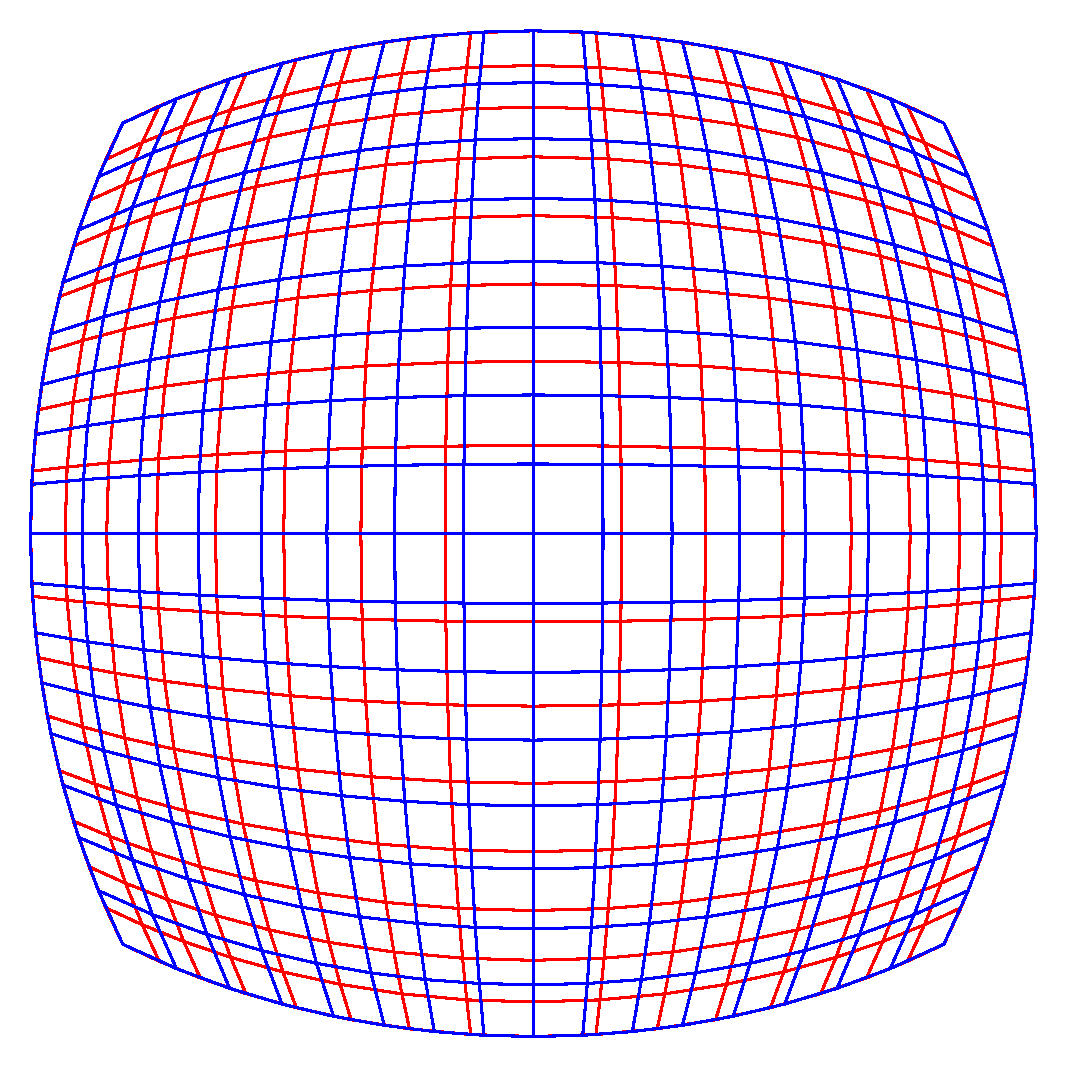
\includegraphics[width=0.3\textwidth]{fig/both.pdf}\label{fig:both}}
  \caption{A comparison of linear and spherical cube map sample uniformity}
  \label{fig:uniformity}
\end{figure}

Similarly, the shortest edge of the linear cube map is only $47\%$ of the length of the longest, while the shortest edge of the spherical cube map is $70\%$ of the length of the longest.\pagenote{Compounding the surprise, the ratio of the length of the shortest edge to the length of the longest edge also tends toward $\sqrt{2}/2$.}  Notably, the vertical and horizontal edges along the center of the \scm\ page all have equal lengths, which means that an \scm\ data set has constant data density along the equator, as well as along the four \ang{90} meridians.

\section{Paging}
\label{sec:paging}

While the \scm\ mapping does a good job of uniformly representing data on the surface of the sphere, we're not content to simply map six large images onto the six faces of an inflated cube. Large images are slow to load, and the ultimate objective of the \scm\ data structure is to support real-time viewing with near-instantaneous data access. To render a multi-giga-pixel spherical data set in real-time, an application must calculate the specific subset of the data visible to the user in each frame, as well as the minimum data resolution necessary to fill all pixels of the user's display. Toward that end, the \scm\ represents a large data set in the form of a number of small pages, at a range of resolutions, organized as a set of six quadtrees.

Cube faces are recursively subdivided, as shown in Figure~\ref{fig:subdivision}, with each four-sided face cut into four child faces, and the newly-created center vertex placed on the surface of the sphere. Each face of the resulting polyhedron gives one spherically-mapped page of image data. A full \scm\ tree gives all levels of detail, up to and including the native resolution of the source data set. The six pages at depth zero (Figure~\ref{fig:cube0}) give low-resolution coverage of the entire sphere. The 24 pages at depth one (Figure~\ref{fig:cube1}) give coverage at twice that density. With each successive increase in depth, the number of pages and the total quantity of image data increases by a factor of four.

\begin{figure}
  \centering
  \subbottom[0]{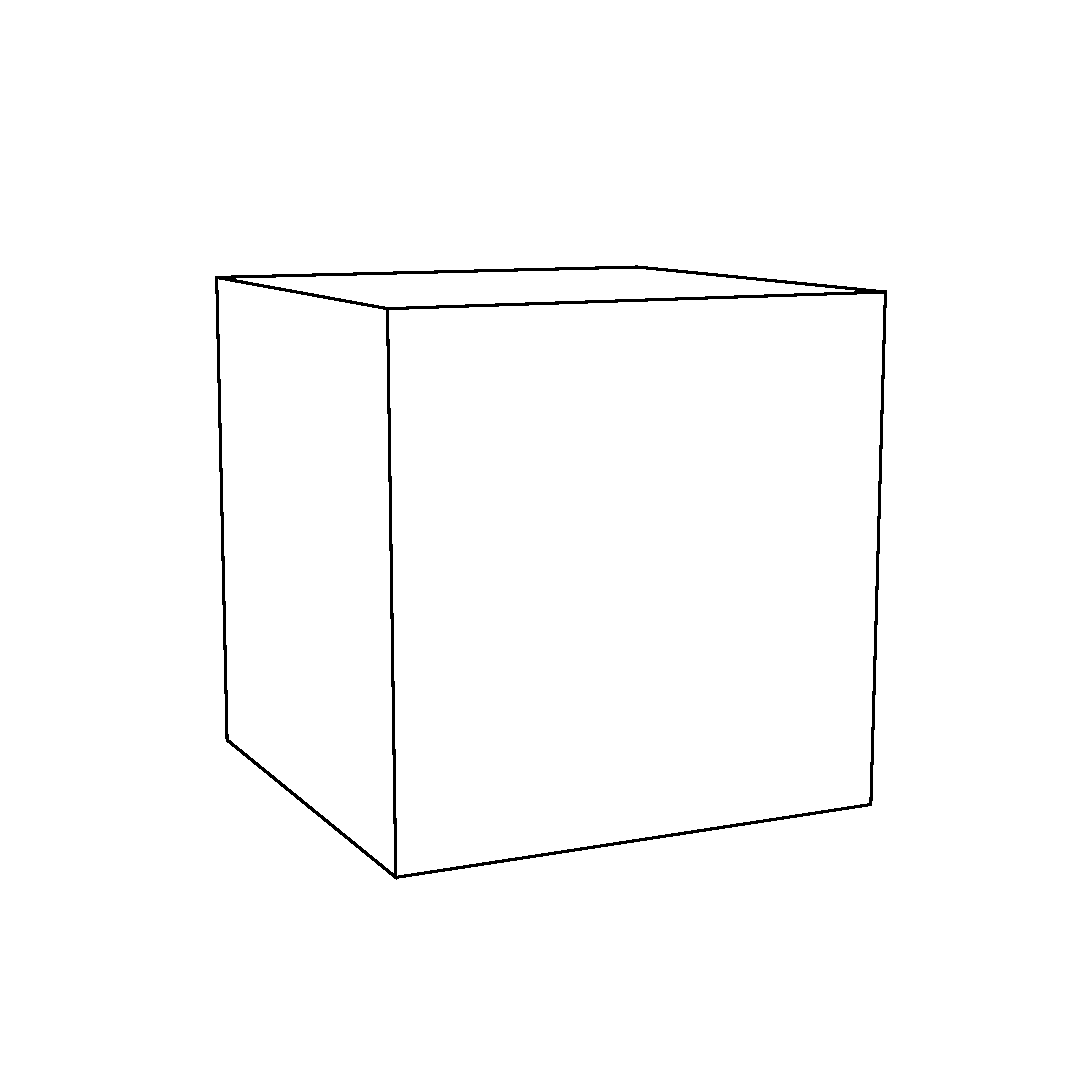
\includegraphics[width=0.18\textwidth]{fig/cube0.pdf}\label{fig:cube0}}
  \subbottom[1]{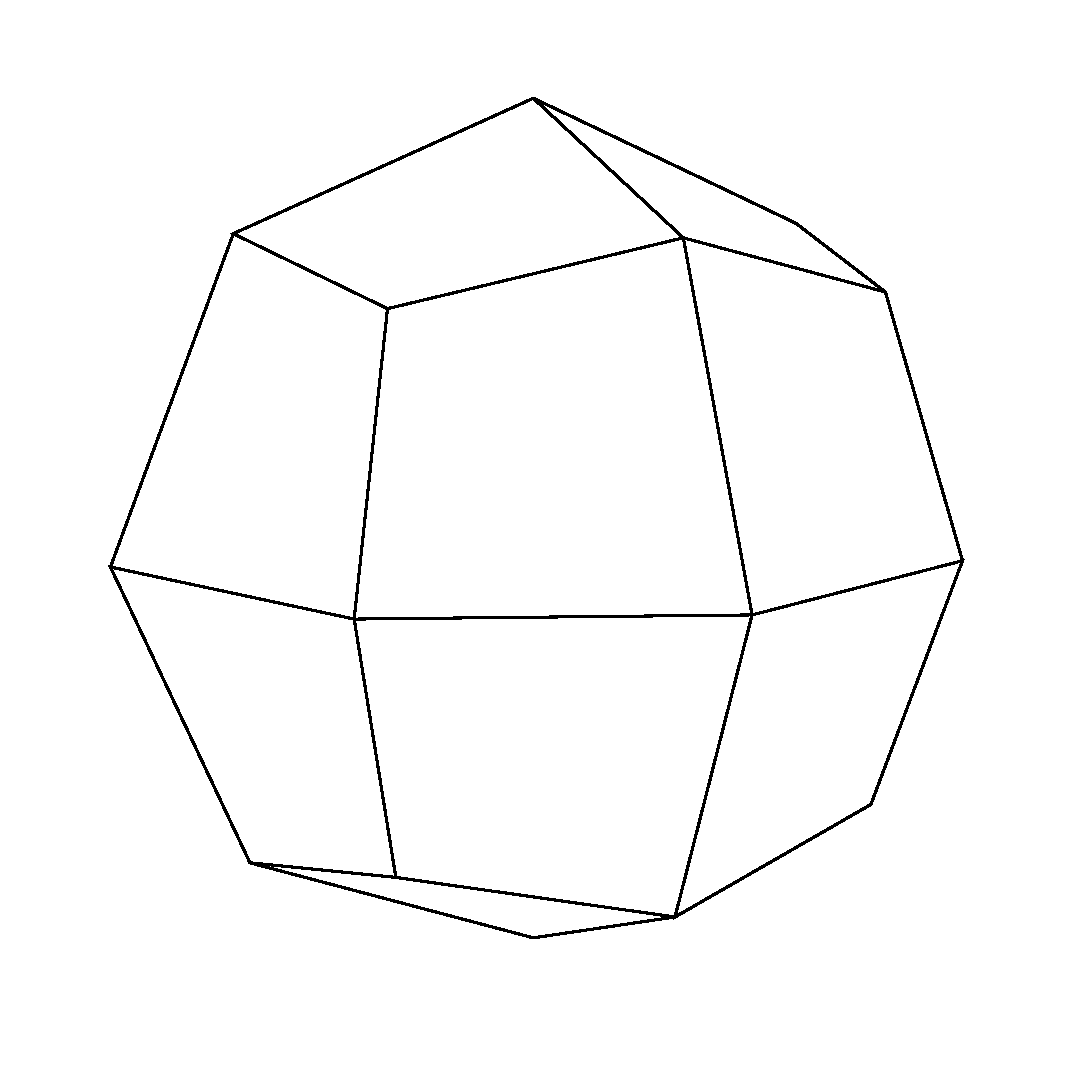
\includegraphics[width=0.18\textwidth]{fig/cube1.pdf}\label{fig:cube1}}
  \subbottom[2]{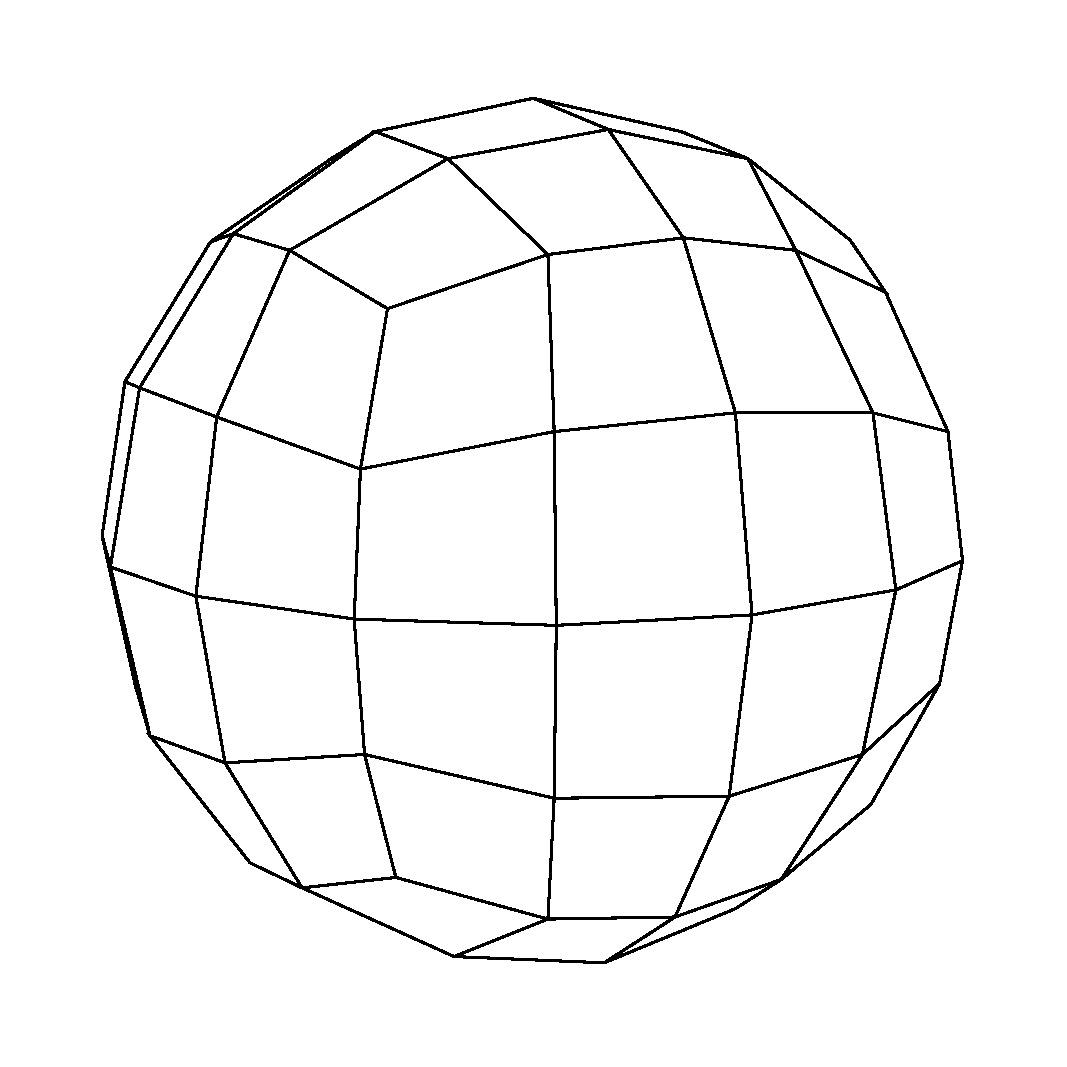
\includegraphics[width=0.18\textwidth]{fig/cube2.pdf}\label{fig:cube2}}
  \subbottom[3]{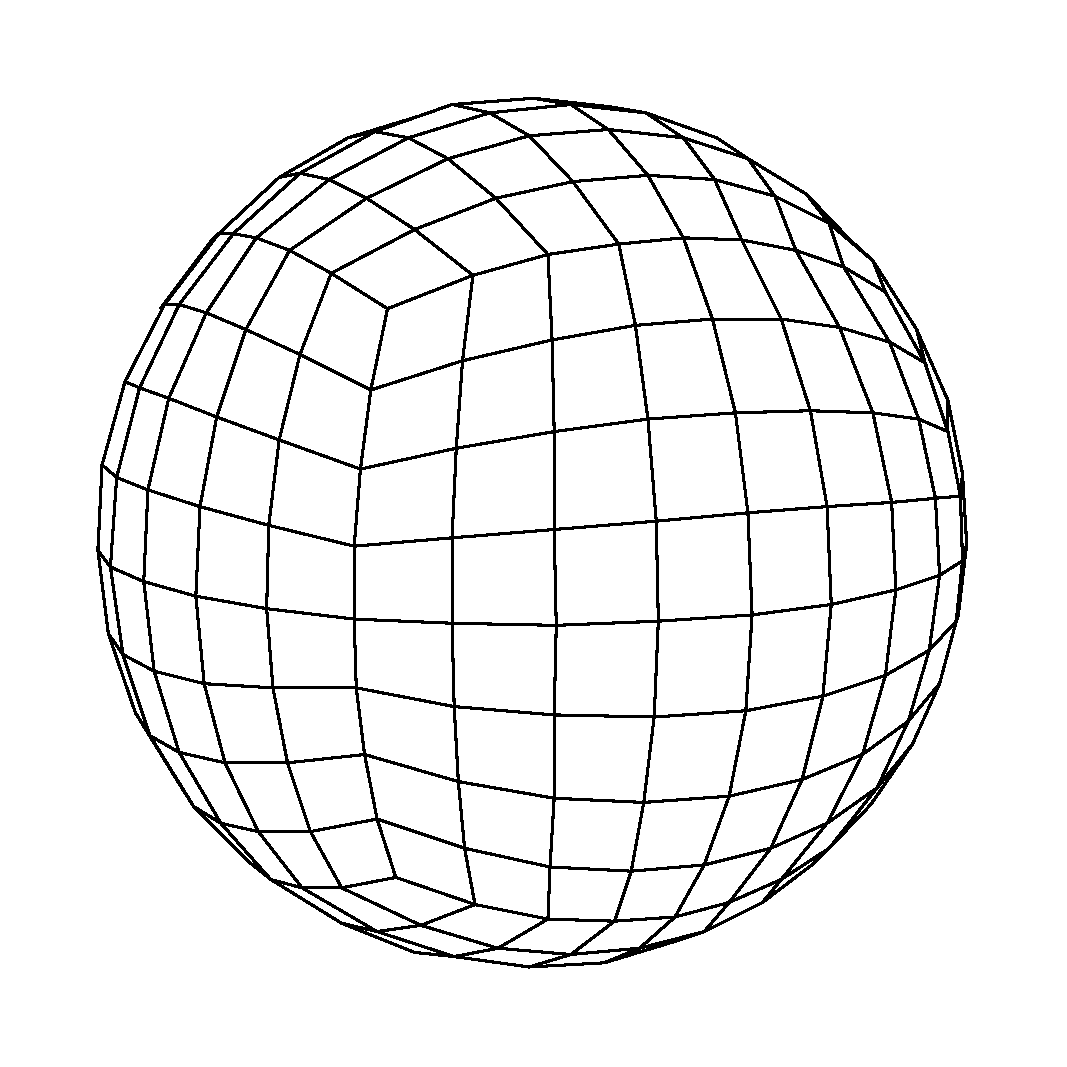
\includegraphics[width=0.18\textwidth]{fig/cube3.pdf}\label{fig:cube3}}
  \subbottom[4]{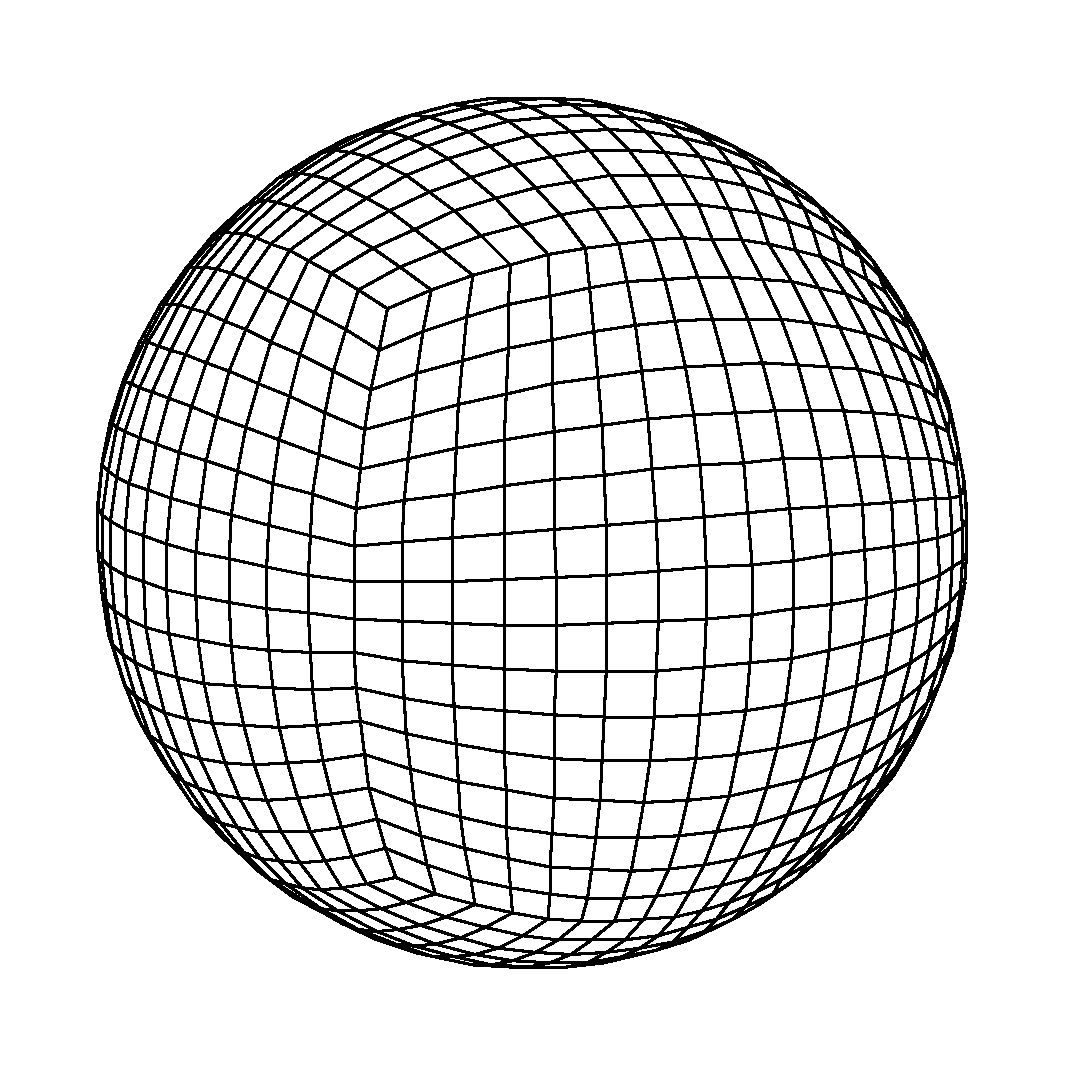
\includegraphics[width=0.18\textwidth]{fig/cube4.pdf}\label{fig:cube4}}
  \hfil
  \caption{Recursive subdivisions of the cube.}
  \label{fig:subdivision}
\end{figure}

Let $d$ be the number of recursive subdivisions applied to the cube. The total number of pages in an \scm\ tree of depth $d$ is
\[\scmcount{d}=2^{2\,d+3}-2.\]

Let $n$ be the size in pixels of each page of image data. The effective sphere map resolution of an \scm\ tree with page size $n$ and depth $d$ is
\[\scmwidth{d}=n\,2^{d+2}\qquad \scmheight{d}=n\,2^{d+1}.\]

For reference, Table~\ref{tab:resolution} shows the effective resolutions and page counts of \scm\ trees with depths down to $7$. Page size $n=512$ is often used for power-of-two source images, and $n=360$ works well for geographic and planetary gridded data.

\begin{table}
  \centering
  \label{tab:resolution}
  \begin{tabular}{r|rr|rr|r}
  $d$& $w_{\,512}$& $h_{\,512}$& $w_{\,360}$& $h_{\,360}$& \textit{count} \B\\\hline
  \num{0}&  \num{2048}&  \num{1024}&  \num{1440}&  \num{720}&     \num{6} \T\\
  \num{1}&  \num{4096}&  \num{2048}&  \num{2880}& \num{1440}&    \num{30} \\
  \num{2}&  \num{8192}&  \num{4096}&  \num{5760}& \num{2880}&   \num{126} \\
  \num{3}& \num{16384}&  \num{8192}& \num{11520}& \num{5760}&   \num{510} \\
  \num{4}& \num{32768}& \num{16384}& \num{23040}&\num{11520}&  \num{2046} \\
  \num{5}& \num{65536}& \num{32768}& \num{46080}&\num{23040}&  \num{8190} \\
  \num{6}&\num{131072}& \num{65536}& \num{92160}&\num{46080}& \num{32766} \\
  \num{7}&\num{262144}&\num{262144}&\num{184320}&\num{92160}&\num{131070} \\
  \end{tabular}
  \caption{Effective resolutions and page counts of \scm\ trees with various depths and page sizes.}
\end{table}

Each page is identified by an index between $0$ and $\scmcount{d}$ giving the page's position in a breadth-first enumeration of the page tree. As with all basic definitions shown so far, this root configuration coincides with the definition of a standard \opengl\ cube map. Pages zero through five map onto the faces of a cube as follows.
\[p_0=+X\quad p_1=-X\quad p_2=+Y\quad p_3=-Y\quad p_4=+Z\quad p_5=-Z\]

The page index uniquely determines all of a page's parameters. Its size, position, and orientation on the sphere, plus its parent, children, and neighbors can all be calculated in constant time given only the page index $i$. The next several equations build the integer arithmetic giving this capability.

The levels of the \scm\ tree are enumerated in increasing order. Within each level, the sub-pages of each root page are contiguous. Thus, each level $\ell$, $0\leq\ell\leq d$ consists of six arrays of $2^\ell\times2^\ell$ pages. The level of a given page $i$ is
\[\scmlevel{i}=\frac{\lfloor\log_2\,(i+2)\rfloor-1}{2}.\]
This integer binary logarithm is used heavily when computing page index relationship, and an efficient C implementation is given in Appendix~\ref{cha:log}.

The root page of a page $i$, its earliest ancestor, is
\[\scmroot{i}=(i-2\,(4^{\scmlevel{i}}-1))\ /\ 4^{\scmlevel{i}}.\]
The pages of the $2^\ell\times 2^\ell$ array for each level and root are enumerated beginning at the top left, going left-to-right and top-to-bottom. The rank of a page in this array is
\[\scmrank{i}=(i-2\,(4^{\scmlevel{i}}-1))\ \%\ 4^{\scmlevel{i}}.\]
Note the use of integer division and modulus, plus the useful symmetry in the definitions of \textit{root} and \textit{rank}. The row and column in the array follow directly from this rank.
\[\scmrow{i}=\scmrank{i}\ /\ 2^{\scmlevel{i}}\]
\[\scmcol{i}=\scmrank{i}\ \%\ 2^{\scmlevel{i}}\]

Given these, the \scm\ spherical mapping defined in Section~\ref{sec:sampling} may be applied, and the \threed\ position vector of each page corner may be determined. To the west and east,
\[\alpha_w=\ang{90}\frac{col(i)}{2^{\scmlevel{i}}}-\ang{45}\quad\textrm{and}\quad
  \alpha_e=\ang{90}\frac{col(i)+1}{2^{\scmlevel{i}}}-\ang{45}.\]
To the north and south,
\[\beta_n=\ang{90}\frac{row(i)}{2^{\scmlevel{i}}}-\ang{45}\quad\textrm{and}\quad
  \beta_s=\ang{90}\frac{row(i)+1}{2^{\scmlevel{i}}}-\ang{45}.\]
The vector pointing toward the north-west corner of page $i$ is thus
\[v_{nw}=\left[\begin{array}{c}
\phantom{-}\sin\alpha_w\, \cos\beta_n\\
        {-}\cos\alpha_w\, \sin\beta_n\\
\phantom{-}\cos\alpha_w\, \cos\beta_n
\end{array}\right],\]
subject to the table of swizzles and negations given in Section~\ref{sec:sampling}. The remaining corners $v_{ne}$, $v_{sw}$, and $v_{se}$ follow accordlingly.

Moving on, just as a page's index uniquely determine its \textit{root}, \textit{level}, \textit{row}, and \textit{col}, so too do these four values together uniquely determine an index.
\[\scmindex{f, \ell, r, c}=\scmcount{\ell-1}+f\,4^\ell+r\,2^\ell+c.\]
Given this two-way set of definitions, parent, child, and neighbor relationships emerge. The parent is one level higher,
\begin{align*}
\scmparent{i}=\scmindex{\scmroot{i}&,\\
                        \scmlevel{i}&-1,\\
                        \scmrow{i}&\ /\ 2,\\
                        \scmcol{i}&\ /\ 2},
\end{align*}
and the four children $0\leq k < 4$ are one level lower,
\begin{align*}
\scmchild{i,k}=\scmindex{\scmroot{i}&,\\
                        \scmlevel{i}&+1,\\
                    2\cdot\scmrow{i}&+k\ /\ 2,\\
                    2\cdot\scmcol{i}&+k\ \%\ 2}.
\end{align*}

The calculation of neighbor indices is a bit more complicated. In the trivial case, the approach is identical to the calculation of a parent or child. One has only to increment or decrement the row or column argument to \scmindex{f,\ell,r,c} to determine any adjacency. However, finding neighbors across cube map face boundaries causes complications due to the varying orientations of the roots. The face swizzle table comes into play and the resulting cases are tedious to derive. They are fully enumerated here for reference and ease of implementation.
\[\scmnorth{f,\ell,r,c}=\mathit{index}\left(
\begin{array}{c}
  f, \\ 2, \\ 2, \\ 5, \\ 4, \\ 2, \\ 2,
\end{array}
\begin{array}{c}
  \ell, \\ \ell, \\ \ell, \\ \ell, \\ \ell, \\ \ell, \\ \ell,
\end{array}
\begin{array}{c}
  r-1, \\ 2^\ell-c-1, \\ c, \\ 0, \\ 2^\ell-1, \\ 2^\ell -1, \\ 0,
\end{array}
\begin{array}{c}
  c \\ 2^\ell-1 \\ 0 \\ 2^\ell-c-1 \\ c \\ c \\ 2^\ell-c-1
\end{array}
\right)
\begin{array}{l}
  \text{if } r > 0 \\
  \text{if } f = 0 \\
  \text{if } f = 1 \\
  \text{if } f = 2 \\
  \text{if } f = 3 \\
  \text{if } f = 4 \\
  \text{if } f = 5
\end{array}\]
%
\[\scmsouth{f,\ell,r,c}=\mathit{index}\left(
\begin{array}{c}
  f, \\ 3, \\ 3, \\ 4, \\ 5, \\ 3, \\ 3,
\end{array}
\begin{array}{c}
  \ell, \\ \ell, \\ \ell, \\ \ell, \\ \ell, \\ \ell, \\ \ell,
\end{array}
\begin{array}{c}
  r+1, \\ c, \\ 2^\ell-c-1, \\ 0, \\ 2^\ell-1, \\ 0, \\ 2^\ell -1,
\end{array}
\begin{array}{c}
  c \\ 2^\ell-1 \\ 0 \\ c \\ 2^\ell-c-1 \\ c \\ 2^\ell-c-1
\end{array}
\right)
\begin{array}{l}
  \text{if } r < 2^\ell \\
  \text{if } f = 0 \\
  \text{if } f = 1 \\
  \text{if } f = 2 \\
  \text{if } f = 3 \\
  \text{if } f = 4 \\
  \text{if } f = 5
\end{array}\]
%
\[\scmwest{f,\ell,r,c}=\mathit{index}\left(
\begin{array}{c}
  f, \\ 4, \\ 5, \\ 1, \\ 1, \\ 1, \\ 0,
\end{array}
\begin{array}{c}
  \ell, \\ \ell, \\ \ell, \\ \ell, \\ \ell, \\ \ell, \\ \ell,
\end{array}
\begin{array}{c}
  r, \\ r, \\ r, \\ 0, \\ 2^\ell-1, \\ r, \\ r,
\end{array}
\begin{array}{c}
  c-1 \\ 2^\ell-1 \\ 2^\ell-1 \\ r \\ 2^\ell-r-1 \\ 2^\ell-1 \\ 2^\ell-1
\end{array}
\right)
\begin{array}{l}
  \text{if } c > 0 \\
  \text{if } f = 0 \\
  \text{if } f = 1 \\
  \text{if } f = 2 \\
  \text{if } f = 3 \\
  \text{if } f = 4 \\
  \text{if } f = 5
\end{array}\]
%
\[\scmeast{f,\ell,r,c}=\mathit{index}\left(
\begin{array}{c}
  f, \\ 5, \\ 4, \\ 0, \\ 0, \\ 0, \\ 1,
\end{array}
\begin{array}{c}
  \ell, \\ \ell, \\ \ell, \\ \ell, \\ \ell, \\ \ell, \\ \ell,
\end{array}
\begin{array}{c}
  r, \\ r, \\ r, \\ 0, \\ 2^\ell-1, \\ r, \\ r,
\end{array}
\begin{array}{c}
  c+1 \\ 0 \\ 0 \\ 2^\ell-r-1 \\ r \\ 0 \\ 0
\end{array}
\right)
\begin{array}{l}
  \text{if } c < 2^\ell \\
  \text{if } f = 0 \\
  \text{if } f = 1 \\
  \text{if } f = 2 \\
  \text{if } f = 3 \\
  \text{if } f = 4 \\
  \text{if } f = 5
\end{array}\]

As shorthand, let $\scmnorth{i} = \scmnorth{\scmroot{i},\scmlevel{i},\scmrow{i},\scmcol{i}}$, etc., and note that our complication has a complication. Due to potential changes in page orientation, diagonal adjacency does not follow directly from nested evaluations of cardinal adjacency. Instead,
\[
\mathit{northwest}(i)=\begin{cases}
\scmnorth{\scmwest{i}} & \text{if } \scmroot{i}=\scmroot{\scmwest{i}} \\
\scmwest{\scmnorth{i}} & \text{otherwise,}\\
\end{cases}
\]
\[
\mathit{northeast}(i)=\begin{cases}
\scmnorth{\scmeast{i}} & \text{if } \scmroot{i}=\scmroot{\scmeast{i}} \\
\scmeast{\scmnorth{i}} & \text{otherwise,}\\
\end{cases}
\]
\[
\mathit{southwest}(i)=\begin{cases}
\scmsouth{\scmwest{i}} & \text{if } \scmroot{i}=\scmroot{\scmwest{i}} \\
\scmwest{\scmsouth{i}} & \text{otherwise,}\\
\end{cases}
\]
\[
\mathit{southeast}(i)=\begin{cases}
\scmsouth{\scmeast{i}} & \text{if } \scmroot{i}=\scmroot{\scmeast{i}} \\
\scmeast{\scmsouth{i}} & \text{otherwise.}\\
\end{cases}
\]

This completes the set of mathematical tools needed to immediately determine all parameters of any \scm\ page.

%------------------------------------------------------------------------------

\chapter{\scm\ Pre-processing}

As a multi-page raster image, An \scm\ tree is naturally amenable to storage in the form of a \tiff\ image file. In this form, \scm\ data is accessible to a variety of existing applications and tools, most notably the \libtiff\ image library.

\section{SCMTIFF}

Spherical data sets in a variety of image formats are converted to \scm\ \tiff\ files by the \scmtiff\ utility. Given the variety of source data preparations, this conversion involves multiple steps, and is often directed by a script or build system. \scmtiff\ is a multi-tool that implements all of the different processes needed when traversing the path from raw data to usable \scm. It takes three global options followed by a list of per-process options and a list of input files.

\bigskip\noindent\scmtiff\ \texttt{-p} \inangles{\textit{process}} [\texttt{-o} \inangles{\textit{output}}] [\textit{options}] \inangles{\textit{input}} [\ldots]

\begin{optionlist}
\item[\texttt{-p} \inangles{\textit{process}}] Selects the \scm\ process. Alternatives include \texttt{convert}, \texttt{combine}, \texttt{mipmap}, \texttt{border}, \texttt{finish}, \texttt{normal}, and \texttt{sample}. Each of these processes is described here, and examples of complete conversions are given below.

\item[\texttt{-o} \inangles{\textit{output}}] Gives the name of the output file. If left unspecified, the default is \texttt{out.tif}, unless otherwise noted.

\item[\texttt{-T}] Requests that process timing be collected and printed to the terminal upon completion.
\end{optionlist}

An \scm\ \tiff\ file produced by the \scmtiff\ tool is a standard \bigtiff\ image, suitable for processing using any \bigtiff-compatible software, including \libtiff\ version 4 or later, and its related utilities.

\subsection{Convert}

\noindent\scmtiff\ \texttt{-p convert} [\texttt{-o} \inangles{\textit{output}}] [\textit{options}] \inangles{\textit{input}} [\ldots]

\bigskip The \texttt{convert} process is the first and most basic, taking source data input and producing \scm\ \tiff\ output. Source data with an equirectangular projection may be provided in \textsc{jpeg}, \textsc{png}, or \textsc{tiff} format, with up to four channels. Data with more complex projection may be provided in \textsc{pds} format, as attached-label \textsc{img} files or detached-label \textsc{lbl}~/~\textsc{img} pairs. Channels may have 8 or 16-bit signed or unsigned integer samples, or 32-bit floating point samples.

If the output file name is not specified using the \texttt{-o} option to \scmtiff, the default name is generated by replacing the file extension of the input file name with \texttt{.tif}. This is important when multiple input files are given on a single command line.\pagenote{Yes, this process is dumb enough to overwrite a source data file that already has the \texttt{.tif} extension.}

\texttt{convert} has the most options of any process, as the parameters specified at the first step are carried through into the final data product.

\begin{optionlist}
\item[\texttt{-n} \inangles{$n$}] Gives a value for $n$, the \scm\ page size. Default is $512$.

\item[\texttt{-d} \inangles{$d$}] Gives a value for $d$, the \scm\ tree depth. Default is $0$. See Section~\ref{paging} for definitions and examples of how the selection of $n$ and $d$ affect image resolution and file size.

\item[\texttt{-b} \inangles{$b$}] Overrides the number of bits per channel. By default, \scmtiff\ uses the bit depth specified by the input image file. If a change in bit depth is desired, this value $b$ is used instead. Values of $8$ and $16$ select integer samples and $32$ selects floating point samples.

\item[\texttt{-g} \inangles{$g$}] Overrides the signedness of integer data. By default, \scmtiff\ uses the type specified by the input file, but if a change is desired, $0$ specifies unsigned and $1$ signed. This option has no effect if floating point samples are selected.

\item[\texttt{-N} \inangles{$n_0$}\texttt{,}\inangles{$n_1$}] Specifies a normalization range. Unsigned integer samples have a natural normalized range of $(0, 1)$, signed integer samples have the normalized range of $(-1,1)$, and floating point samples have the full range of a 32-bit float. This option remaps each sample onto the range $(n_0,n_1)$. The choice of normalization depends largely on the character of the input and the type of the output. The default normalization retains the natural range of the data.

\item[\texttt{-E} \inangles{$w$}\texttt{,}\inangles{$e$}\texttt{,}\inangles{$s$}\texttt{,}\inangles{$n$}] Specifies a range for equirectangular inputs \textit{other than} \textsc{pds}. This allows a \textsc{jpeg}, \textsc{png}, or \textsc{tiff} to represent a subset of the sphere. The default is $0^{\circ}$, $360^{\circ}$, $-90^{\circ}$, $90^{\circ}$.

\item[\texttt{-L} \inangles{$\lambda_c$}\texttt{,}\inangles{$\lambda_0$}\texttt{,}\inangles{$\lambda_1$}] Specifies a longitudinal mask. This causes data to appear over a given range of longitudes, fading out at the edges, thus allowing the blended combination of separate source data files. This option chooses a range of degrees centered at $\lambda_c$, extending to $\lambda_c\pm\lambda_1$, and fading with cubic drop-off to $\lambda_c\pm\lambda_0$.

\item[\texttt{-P} \inangles{$\phi_c$}\texttt{,}\inangles{$\phi_0$}\texttt{,}\inangles{$\phi_1$}] Specifies a latitudinal mask. This option chooses a range of degrees centered at $\phi_c$, extending to $\phi_c\pm\phi_1$, and fading with cubic drop-off to $\phi_c\pm\phi_0$. Longitudinal and latitudinal masks may be applied simultaneously.
\end{optionlist}

\subsection{Combine}

\noindent\scmtiff\ \texttt{-p combine} [\texttt{-o} \inangles{\textit{output}}] [\textit{options}] \inangles{\textit{input}} [\ldots]

\bigskip The \texttt{combine} process is the second step in cases where a data set is provided in a form spread across multiple data file. It merges multiple converted \scm\ \tiff\ input files into a single \scm\ \tiff\ output file. It takes just one optional argument.

\begin{optionlist}
\item[\texttt{-m} \inangles{\textit{mode}}] Specifies the operator mode used to combine samples. The \texttt{max} mode selects the largest sample from each of the named files. The \texttt{sum} mode is the default and sums all named files. The \texttt{max} mode is often used when merging data sets of differing projection, while the \texttt{sum} mode is used when combining data sets that have had a longitudinal or latitudinal mask applied in the \texttt{convert} process.
\end{optionlist}

\subsection{Mipmap}

\noindent\scmtiff\ \texttt{-p mipmap} \inangles{\textit{input}}

\bigskip The \texttt{mipmap} process generates the intermediate nodes of an \scm\ tree. In general, the \texttt{convert} process generates tree leaves, the \texttt{combine} process merges trees, and the \texttt{mapmap} process subsamples the result, enabling real-time display of the data at arbitrary resolution. It is important to \texttt{combine} before \texttt{mipmap}ping, as boundary artifacts may remain apparent in the intermediate pages of combined mipmaps.

The \texttt{mipmap} process takes no parameters. In the interest of efficiency, mipmapping occurs \textit{in place}. The output file name option is ignored and subsampled pages are appended to the existing file. The \texttt{mipmap} process generates as many subsampled levels as possible, and in the common case, an input with depth $d$ will have $d-1$ levels appended to it.

\subsection{Border}

\noindent\scmtiff\ \texttt{-p border} [\texttt{-o} \inangles{\textit{output}}] \inangles{\textit{input}}

\bigskip In truth, an \scm\ with page size $n$ is stored in a \tiff\ file with image width and height $n+2$. The \texttt{border} process fills these extra pixels in the outermost rows and columns of each page with pixels from the adjacent rows or columns of the four neighboring pages. This provides each page with the context needed by the graphics hardware to perform linear magnification filtering across page boundaries, effectively allowing many small images to appear as a single very large image.\pagenote{The replicated borders provide only a single pixel of context. This enables linear magnification filtering, but does \emph{not} enable anisotropic filtering.} If this step is not performed, artifacts will appear in the output. In practice, the \texttt{border} process is expensive, as it must decompress and recompress every page of the \scm.

\subsection{Finish}

\noindent\scmtiff\ \texttt{-p finish} [\textit{options}] \inangles{\textit{input}}

\bigskip The \texttt{finish} process calculates and appends \scm\ metadata for the given \scm\ \tiff\ file. This metadata is three-fold: offsets, bounds, and description.

\begin{enumerate}
\item A sorted array of page indices and file offsets allows an \scm\ rendering application to immediately determine exactly where each page appears in the \scm\ \tiff\ file. Given an awareness of how points on the sphere map onto indices, the page catalog generated by the \texttt{finish} process allows applications to straightforwardly locate the unique \scm\ \tiff\ data that maps onto any point on the sphere at any resolution.

\item The minimum and maximum values of each channel of each page allow a displacement-mapping application to determine a tight \threed\ bounding volume for each page. This enables efficient visibility determination and view culling.

\item An image description documents the provenance of an image, noting its source and copyright holder.
\end{enumerate}

Like mipmapping, the \texttt{finish} process occurs \emph{in place}. The output file name option is ignored and the generated data is appended to the input file.

\begin{optionlist}
\item[\texttt{-t} \inangles{\textit{file}}] Specifies a text file containing an image description. The contents of this file are read and embedded in the generated \tiff\ file.

\item[\texttt{-l} \inangles{$\ell$}] Specifies a \emph{leaf subdivision depth}. This argument allows the depth of the bounding value cache hierarchy to exceed the depth of the actual page hierarchy. The rationale for this feature is complex, but as we will see in Section~\ref{sec:scmxml}, there is a mismatch between the resolution of a displacement map and the mesh geometry that it displaces. Leaf subdivision accounts for this mismatch. As a rule of thumb, $\ell$ should give the base-two logarithm of the mesh's down-sampling factor. For example, when finishing a $512\times 512$ displacement map for display on a $128\times 128$ mesh, $\log_2\, 512 / 128=2$, so specify $\ell=2$. For most imagery, leaf subdivision is not beneficial, and the default value of zero should be used.
\end{optionlist}

\subsection{Normal}

\noindent\scmtiff\ \texttt{-p normal} [\texttt{-o} \inangles{\textit{output}}] [\textit{options}] \inangles{\textit{input}}

\bigskip The \texttt{normal} process computes a normal map for a given height map. The input may have any number of channels and any format, but only the first channel is used, and the normalization of that channel is modified by the range of radii specified by the command line option. The output will always have 3 channels of 8-bit unsigned samples, scaled and biased to $(0,1)$ as is standard practice in normal mapping, though the normals are given in \emph{object} space rather than \emph{tangent} space.

Regardless of whether the input height map was bordered or finished, the output normal map will be neither bordered nor finished. In contrast, a mipmapped input height map \emph{will} produce a mipmapped normal map output, and indeed one should \emph{always} normalize mipmaps instead of mipmapping normals, as a mipmapped normal is not guaranteed to have unit length.

\begin{optionlist}
\item[\texttt{-R} \inangles{$r_0$}\texttt{,}\inangles{$r_1$}] Specifies the true range of radii represented by the normalized height map input. This allows the true magnitude of the \emph{change} in height to be computed, which gives slope, which gives the normal vector.
\end{optionlist}

\subsection{Sample}

\noindent\scmtiff\ \texttt{-p sample} [\textit{options}] \inangles{\textit{input}}

\bigskip The \texttt{sample} process is not a tool for preprocessing \scm\ data, but for working with already-processed data. It queries the contents of the \scm\ \tiff\ file named on the command line, and produces no new \scm\ \tiff\ output. The \texttt{sample} process receives queries as latitude-longitude pairs, in degrees, on \texttt{stdin}. It reports the results on \texttt{stdout}.

\begin{optionlist}
\item[\texttt{-R} \inangles{$r_0$}\texttt{,}\inangles{$r_1$}] Specifies the true range of radii represented by the input. This allows the magnitude of the query to be correctly reported, even if the data has been renormalized during the \texttt{convert} process.
\end{optionlist}

For example, to query the radius in meters of the landing point of Apollo 16, as given by the merged lunar heightmap prepared in the example of Section~\ref{sec:planet}:

\begin{Verbatim}
echo "-8.973 15.500" | scmtiff -p sample -R 1728240,1748170 DTM.tif
1737382.875000
\end{Verbatim}

The \texttt{sample} process does \emph{not} expect a finished \scm\ and will perform a scan of the \scm\ \tiff\ file prior to responding to queries. Thus the very first query may take a few moments to process, while subsequent queries will process immediately. If many queries are to be made, the best practice is to concatenate them in a file.

\section{SCMVIEW}

The \scmview\ utility enables interactive inspection and side-by-side comparison of individual pages of \scm\ \tiff\ files. Figure~\ref{fig:scmview} shows a screenshot of \scmview\ in action. There, four \scm\ files are displayed together, with their pan, zoom, and page number in sync. The user has focused upon Clavius, a region of interest on a lunar height map. The first frame shows a converted equirectangular projection of the map, the second shows a polar projection, and the third demonstrates their seamless merger. This output is taken from the usage example of Section~\ref{sec:planet}. The fourth frame shows a normal map derived from the merged height map, discussed in Section~\ref{sec:normal}.

\begin{figure}
  \centering
  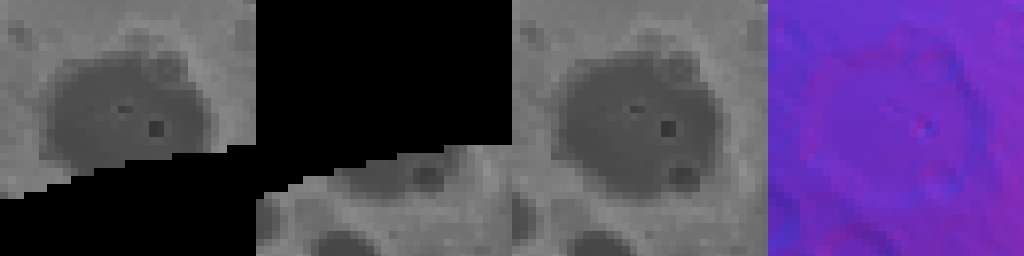
\includegraphics[width=\textwidth]{fig/scmview.png}
  \caption{The \scmview\ utility displaying four of the outputs of the conversion described in Sections~\ref{sec:planet} and ~\ref{sec:normal}.}
  \label{fig:scmview}
\end{figure}

The \scmview\ utility takes a list of \scm\ \tiff\ files on the command line.

\bigskip\noindent\scmview\ [\inangles{\textit{GLUT options}}] \inangles{\textit{input}} [\ldots]

\bigskip Keyboard and mouse inputs are as follows.

\begin{optionlist}
\item[Left Mouse] \ldots\ Click and drag to pan.
\item[Right Mouse] \ldots\ Click and drag to zoom.
\item[Return] \ldots\ Reset the pan and zoom.
\item[Page Up] \ldots\ Go to the next page.
\item[Page Down] \ldots\ Go to the previous page.
\item[Shift Page Up] \ldots\ Scan for the next present page.
\item[Shift Page Down] \ldots\ Scan for the previous present page.
\item[{\setlength{\arraycolsep}{0pt}
$\begin{array}{ccc}
\X{7} & \X{ }      & \X{9} \\[-5pt]
\X{ } & \X{\times} & \X{ } \\[-5pt]
\X{1} & \X{ }      & \X{3} \\
\end{array}$
}] \ldots\ Go to one of the four child pages.
\item[{\setlength{\arraycolsep}{0pt}
$\begin{array}{ccc}
\X{ } & \X{8} & \X{ } \\[-2pt]
\X{4} & \X{+} & \X{6} \\[-2pt]
\X{ } & \X{2} & \X{ } \\
\end{array}$
}] \ldots\ Go to one of the four neighbor pages.
\item[5] \dots\ Go to the parent page.
\item[0] \dots\ Go to the root page.
\item[F1] \ldots\ Normal view mode.
\item[F2] \ldots\ False color view mode.
\item[Escape] \ldots\ Exit.
\end{optionlist}

\scmview\ is a \textsc{GLUT} application, and as such it takes the usual set of \textsc{GLUT} command line options. The most useful of these is

\begin{optionlist}
\item[\texttt{-geometry} \inangles{$w$}\texttt{x}\inangles{$h$}] Display a window with size $(w, h)$.
\end{optionlist}

\section{Examples}

\subsection{A Basic Panorama}
\label{sec:panorama}

The most straightforward \scm\ \tiff\ process uses a single image file giving an equirectangular spherical projection, such as that shown in Figure~\ref{fig:bluebonnet}. This image is $\num{32768}\times\num{16384}$ with 3 channels of 8-bit unsigned samples. The name \texttt{Bluebonnet-0-L.tif} reflects that it was captured at the Bluebonnet Swamp Nature Center, it was the first of several captures, and it gives the left channel of a stereoscopic pair.

\begin{figure}
  \centering
  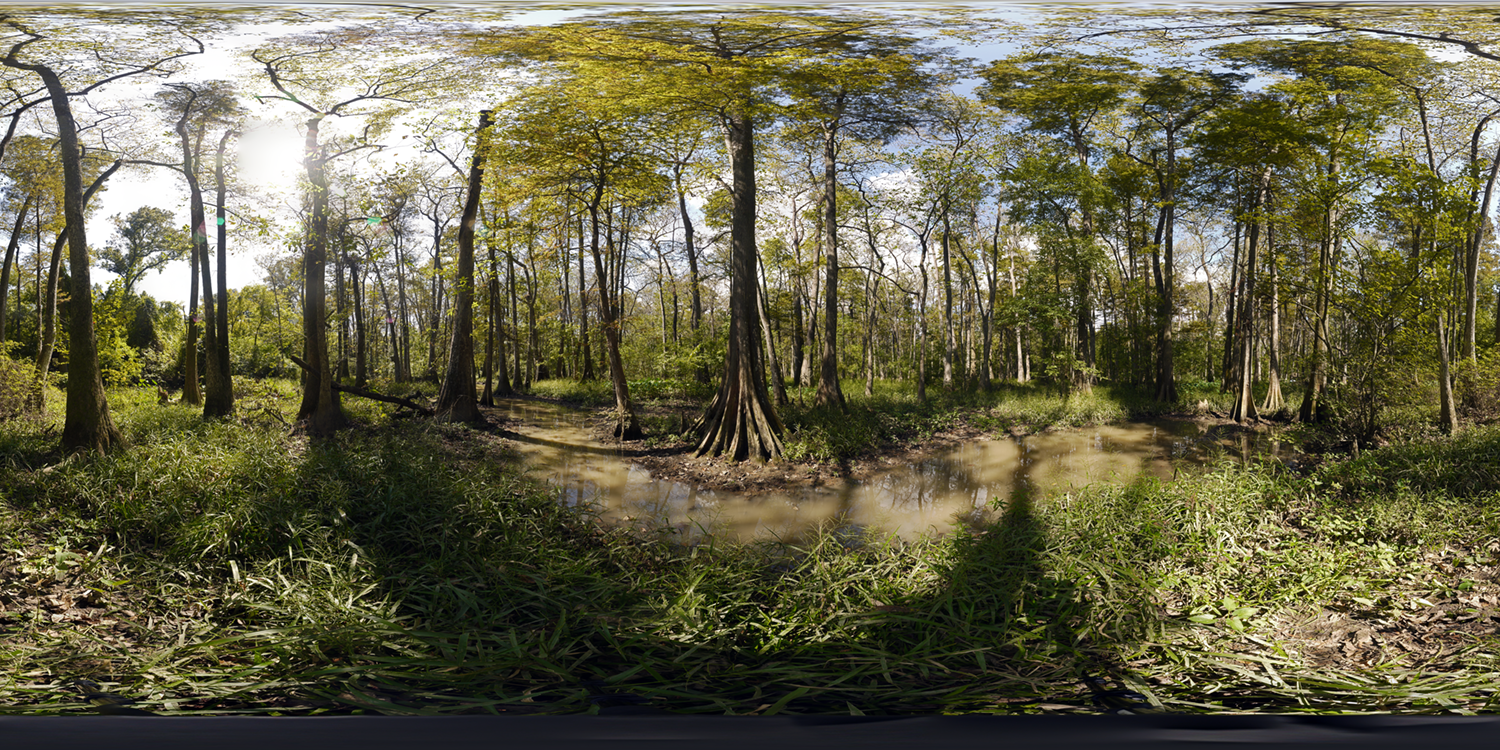
\includegraphics[width=\textwidth]{fig/bluebonnet.png}
  \caption{\texttt{Bluebonnet-0-L.tif}, an equirectangular full-sphere panorama}
  \label{fig:bluebonnet}
\end{figure}

Table~\ref{tab:resolution} indicates that an image with this resolution is well-represented by an \scm\ with page size $n=512$ and depth $d=4$. When finished, the \scm\ tree will have $2046$ pages. The first step is to run the \texttt{convert} process to generate the leaves of this tree. The output file name is chosen to reflect the parameters of the \scm\ as well as the state of its processing. This convention is optional.

\begin{Verbatim}
scmtiff -p convert -n 512 -d 4 -o Bluebonnet-0-L-512-4-M.tif \
                                  Bluebonnet-0-L.tif
\end{Verbatim}

If the output is examined using \scmview, pages $510$ through $2045$ will be present with a resolution of $514\times 514$. Image detail will closely reflect that of the input. There will be mild projection distortion apparent in some pages, though the degree of distortion will be far less than that at the top and bottom of the equirectangular input. All pages will have a border of black pixels around the outside.

The second step is to run the \texttt{mipmap} process on this output to generate the intermediate, subsampled pages.

\begin{Verbatim}
scmtiff -p mipmap Bluebonnet-0-L-512-4-M.tif
\end{Verbatim}

Examination with \scmview\ will show that pages $0$ through $2045$ are now all present. Pages $0$ through $5$ will show full views along each of the axes, and pages $2$ and $3$ will show nicely recovered polar views with all of the projection distortion in the input rectified.

The third step fills the border pixels with adjacent page information. This process alters the compressed size of each page, so it cannot be performed in-place. An output file name is required and a new \scm\ \tiff\ file is generated.

\begin{Verbatim}
scmtiff -p border -o Bluebonnet-0-L-512-4.tif \
                     Bluebonnet-0-L-512-4-M.tif
\end{Verbatim}

The output is a complete \scm\ tree. Figure~\ref{fig:sixfaces} shows the first six pages of output generated from the input in Figure~\ref{fig:bluebonnet}.

\begin{figure}
  \centering
  
\includegraphics[width=0.24\textwidth]{fig/blank.pdf}
  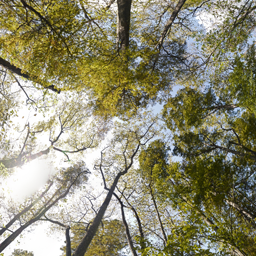
\includegraphics[width=0.24\textwidth]{fig/bluebonnet2.png}
  
\includegraphics[width=0.24\textwidth]{fig/blank.pdf}
  
\includegraphics[width=0.24\textwidth]{fig/blank.pdf}\\\vspace{1pt}
  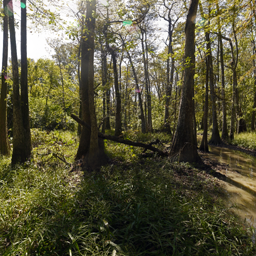
\includegraphics[width=0.24\textwidth]{fig/bluebonnet0.png}
  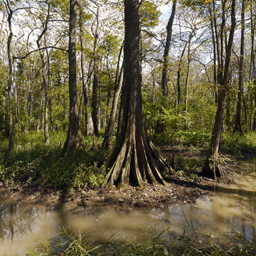
\includegraphics[width=0.24\textwidth]{fig/bluebonnet5.png}
  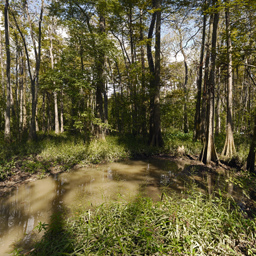
\includegraphics[width=0.24\textwidth]{fig/bluebonnet1.png}
  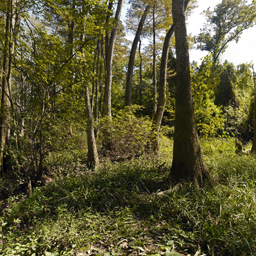
\includegraphics[width=0.24\textwidth]{fig/bluebonnet4.png}\\\vspace{1pt}
  
\includegraphics[width=0.24\textwidth]{fig/blank.pdf}
  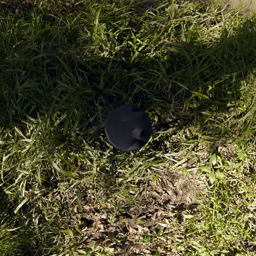
\includegraphics[width=0.24\textwidth]{fig/bluebonnet3.png}
  
\includegraphics[width=0.24\textwidth]{fig/blank.pdf}
  
\includegraphics[width=0.24\textwidth]{fig/blank.pdf}
  \caption{The six root pages of the Bluebonnet \scm.}
  \label{fig:sixfaces}
\end{figure}

The fourth and final step scans the file, noting the location and bounds of each page, and appending this information to the end of the file. With this, a real-time interactive application, such as the one described in the next chapter, can instantly locate, load, and display any page. A brief description is added to an ASCII text file named \texttt{desc.txt},
%
\begin{Verbatim}
Bluebonnet Swamp Nature Center - 9 October 2011
Copyright (c) 2011 Robert Kooima
\end{Verbatim}
%
and the \scm\ \tiff\ is finished.
%
\begin{Verbatim}
scmtiff -p finish -t desc.txt Bluebonnet-0-L-512-4.tif
\end{Verbatim}

\subsection{A Merged Planetary Dataset}
\label{sec:planet}

The following example is much more involved, merging multiple data sets captured by the Lunar Reconnaissance Orbiter (LRO) to produce a globally-high-quality height map of the moon. Deriving this process requires a close familiarity with the source data, and a great deal of trial and error. However, this does represent real-world data handling and usage of \scmtiff.

The LRO height map is based primarily on a 100 meter-per-pixel digital terrain model (DTM) derived by stereo reconstruction from imagery captured by the Wide Angle Camera (WAC) of the Lunar Reconnaissance Orbiter Camera (LROC).\pagenote{\url{http://wms.lroc.asu.edu/lroc/global_product/100_mpp_DEM}} This data set, known as the Global Lunar 100 Meter DTM (GLD100), gives beautifully clean terrain data over most of the moon, omitting only the poles, where illumination and stereo disparity are insufficient for reconstruction.

\begin{figure}
  \centering
  \subbottom[GLD E300N0450]{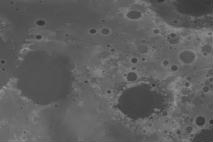
\includegraphics[width=0.24\textwidth]{fig/WAC_GLD100_E300N0450.jpg}}
  \subbottom[GLD E300N1350]{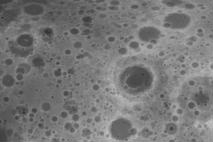
\includegraphics[width=0.24\textwidth]{fig/WAC_GLD100_E300N1350.jpg}}
  \subbottom[GLD E300N2250]{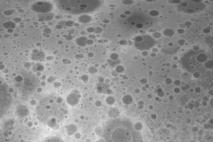
\includegraphics[width=0.24\textwidth]{fig/WAC_GLD100_E300N2250.jpg}}
  \subbottom[GLD E300N3150]{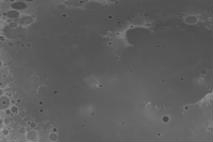
\includegraphics[width=0.24\textwidth]{fig/WAC_GLD100_E300N3150.jpg}}\\
  \subbottom[GLD E300S0450]{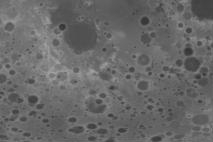
\includegraphics[width=0.24\textwidth]{fig/WAC_GLD100_E300S0450.jpg}}
  \subbottom[GLD E300S1350]{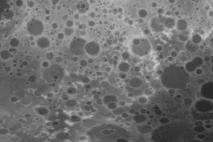
\includegraphics[width=0.24\textwidth]{fig/WAC_GLD100_E300S1350.jpg}}
  \subbottom[GLD E300S2250]{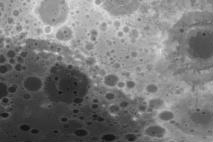
\includegraphics[width=0.24\textwidth]{fig/WAC_GLD100_E300S2250.jpg}}
  \subbottom[GLD E300S3150]{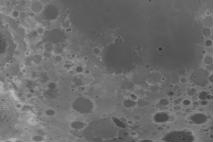
\includegraphics[width=0.24\textwidth]{fig/WAC_GLD100_E300S3150.jpg}}
  \caption{The eight equirectangular projections of GLD100.}
  \label{fig:glde}
\end{figure}

In the interest of optimal image representation, GLD100 is provided in several parts, with two different projections. Latitudes below \ang{60} are given by eight equirectangular projections, shown in Figure~\ref{fig:glde}. Each of these is $\num{27291}\times\num{18195}$ pixels in size, totaling $\num{109164}\times\num{36390}$ pixels. Latitudes above \ang{60} are given by two stereographic polar projections, shown in Figures~\ref{fig:gldn} and~\ref{fig:glds}. Latitudes beyond \ang{79} are not represented.

Fortunately, GLD100 is registered with the Lunar Digital Elevation Model (LDEM) captured by the Lunar Orbiter Laser Altimeter (LOLA).\pagenote{\url{http://pds-geosciences.wustl.edu/missions/lro/lola.htm}} Due to the polar orbit of LRO and the incredibly narrow field of view of LOLA, the coverage of LDEM is very sparse at low latitudes, but excellent near the poles. GLD and LDEM compliment one another in this regard, and we can use the latter to fill the gaps in the former. Figures~\ref{fig:lolan} and~\ref{fig:lolas} show polar projections of LDEM that align with those of GLD. In general, GLD is preferred to LDEM as the coverage and character of stereo reconstructed data is superior to laser altimetry data.

\begin{figure}
  \centering
  \subbottom[GLD P900N0000\label{fig:gldn}]{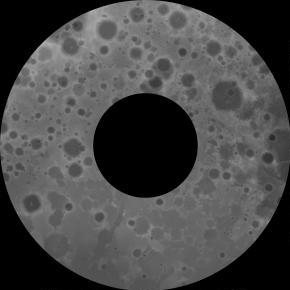
\includegraphics[width=0.24\textwidth]{fig/WAC_GLD100_P900N0000.jpg}}
  \subbottom[GLD P900S0000\label{fig:glds}]{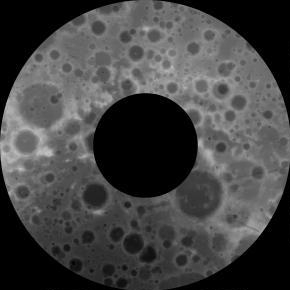
\includegraphics[width=0.24\textwidth]{fig/WAC_GLD100_P900S0000.jpg}}
  \subbottom[LDEM 60N\label{fig:lolan}]{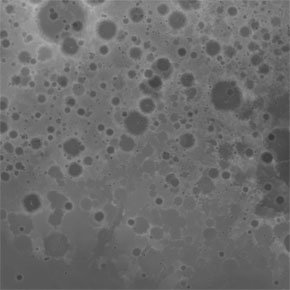
\includegraphics[width=0.24\textwidth]{fig/ldem_60n.jpg}}
  \subbottom[LDEM 60S\label{fig:lolas}]{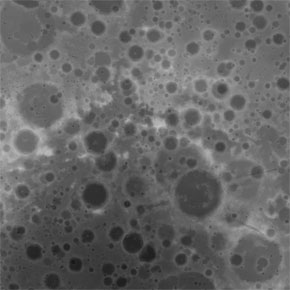
\includegraphics[width=0.24\textwidth]{fig/ldem_60s.jpg}}
  \caption{The two polar projections of GLD100 and LDEM.}
  \label{fig:gldp}
\end{figure}

We need to select a page size and tree depth appropriate for this data set. There are many considerations.

\begin{enumerate}
\item To properly represent the source data, we select $n$ and $d$ such that the effective width, $w=n\,2^{d+2}$, closely matches the total horizontal resolution of the input.

\item Large $n$ incurs high I/O latency. RAM-to-VRAM data transfers take time, and if a page upload consumes a significant fraction of a frame period then the frame rate is likely to break up during high I/O load. Given 2012 era hardware, we'll want $n$ around $512$.

\item For a given $w$, small $n$ requires large $d$. This increases the total number of pages in flight at any given moment, as well as the number of texture image units consumed by the renderer. This is usually not a problem, but depending upon the hardware, one may encounter a limit.\pagenote{The real limit is the total depth of all simultaneously loaded data sets, which must be less than GL\_MAX\_TEXTURE\_IMAGE\_UNITS. On a 2012-era Mac, this limit is 16. On a 2012-era NVIDIA-equipped Linux or Windows PC, this limit is 56 or 64.}

\item The page granularity of a height map impacts the effectiveness of visibility testing, as small pages allow tighter bounding volumes than large pages. This consideration does not apply to color maps or normal maps.

\item $n$ should be an even number to ensure no artifacts arise during the mipmapping process.
\end{enumerate}

Given $w=\num{109164}$, arbitrarily choosing $d=5$, and solving, we find $n=852$. That's quite high. Choosing $d=6$, we find $n=426$, which is reasonable from most perspectives. \scm\ parameters $n=426$ and $d=6$ will give an effective resolution of $\num{109056}\times\num{54528}$ in $\num{32766}$ pages. This is a couple pixels short, but very close to perfect.

It's important to remember that an \scm\ data product is essentially a temporary cache for visualization. It's not a permanent archive, so source integrity need not be considered precious and we're free to renormalize. This will let us benefit from any smoothing that occurs during resampling and reprojection and take full advantage of the output bit depth. Both GLD and LDEM are signed 16-bit samples ranging from roughly \SI{-9160}{\meter} to \SI{10770}{\meter}, giving height values relative to the moon's average radius of \SI{1737400}{\meter}. These values give our normalization range. Of course, normalization maps the data onto $(0,1)$, so there's no longer any point in using a signed sample, so we'll override the \img\ data type and force unsigned output.

Given these parameters, the conversion of the equirectangular inputs of Figure~\ref{fig:glde} is as follows.

\begin{Verbatim}
scmtiff -p convert -n 426 -d 6 -N -9160,10770 -g 0 WAC_GLD100_*.IMG
\end{Verbatim}

The eight output \scm s will be combined using the \texttt{sum} operator. This best accommodates the behavior of edge pixels during resampling and reprojection, as an \scm\ sample falling only partially within the bounds of an \img\ has a coverage coefficient applied. To clarify this point, if the \scm\ sample \emph{should} be $1.0$, but only $20\%$ of the sample falls within the \img, then the sample value will be $0.2$. This does \emph{not} cause edge artifacts because the adjacent \img s may be expected to cover the remainder of the sample, and their contributions will sum to $1.0$. Next we will see a case where this assumption fails, so we must write the summed combination of all equirectangular GLD inputs to a temporary file. We'll call it \texttt{DTM-E.tif}.

\begin{Verbatim}
scmtiff -p combine -o DTM-E.tif WAC_GLD100_*.tif
\end{Verbatim}

The polar GLD inputs of Figures~\ref{fig:gldn} and~\ref{fig:glds} have a different projection so they are not pixel-aligned with the equirectangular inputs. They overlap slightly and the coverages sum to more than $1.0$. Careful scrutiny with \scmview, as in Figure~\ref{fig:scmview}, can reveal issues like this, but usually they only became apparent as flaws in the output. To resolve the issue, the polar inputs will be combined with the already-merged equatorial inputs using the \texttt{max} operator.

But before that can be done, we must look ahead to the contribution of LDEM. As apparent in Figure~\ref{fig:gldp}, GLD and LDEM overlap \emph{heavily}. Due to the vastly different processes that captured them, they have very different character at full resolution. In an effort to obscure any discontinuity that might emerge at their border, we interpolate from one to the other between \ang{78} and \ang{79} degrees. This is accomplished using a latitudinal fade during the initial conversion from \img\ to \scm. Here, the northern annulus of GLD data begins to fade out within \ang{11} of the north pole at \ang{90}, and fades out completely within \ang{12} of \ang{90}.

\begin{Verbatim}
scmtiff -p convert -n 426 -d 6 -N -9160,10770 -g 0 \
        -P 90,12,11 WAC_GLD100_P900N0000.IMG
\end{Verbatim}

The opposite is true for the northern cap of LDEM. It begins to fade in within \ang{11} of \ang{90} and fades in completely within \ang{12} of \ang{90}.

\begin{Verbatim}
scmtiff -p convert -n 426 -d 6 -N -9160,10770 -g 0 \
        -P 90,11,12 ldem_45n_100m.lbl
\end{Verbatim}

The situation at the south pole is the same, but centered upon \ang{-90}.

\begin{Verbatim}
scmtiff -p convert -n 426 -d 6 -N -9160,10770 -g 0 \
        -P -90,12,11 WAC_GLD100_P900S0000.IMG
scmtiff -p convert -n 426 -d 6 -N -9160,10770 -g 0 \
        -P -90,11,12 ldem_45s_100m.lbl
\end{Verbatim}

When these \scm\ files are summed, no discontinuity will be apparent. We write this combination of all polar data to a temporary file named \texttt{DTM-P.tif}.

\begin{Verbatim}
scmtiff -p combine -o DTM-P.tif WAC_GLD100_P*.tif ldem_45*.tif
\end{Verbatim}

To complete the merger of the inputs, it remains only to combine the equirectangular and polar data sets using the max operator. As suggested above, a slight overlap between the two exists. It is too thin for interpolation, yet too thick to go unnoticed when summed.

\begin{Verbatim}
scmtiff -p combine -m max -o DTM-M.tif DTM-E.tif DTM-P.tif
\end{Verbatim}

And with that, the leaves of the \scm\ are in place. We mipmap, border, and finish just as before to arrive at a usable data product.

\begin{Verbatim}
scmtiff -p mipmap DTM-M.tif
scmtiff -p border -o DTM.tif DTM-M.tif
scmtiff -p finish DTM.tif
\end{Verbatim}

The six root pages of this \scm\ are shown in Figure~\ref{fig:dtmh}. Note, in particular, the top and bottom pages, both of which seamlessly combine interpolations of different data sets as well as mergers of distinct projections.

\begin{figure}
  \centering
  
\includegraphics[width=0.24\textwidth]{fig/blank.pdf}
  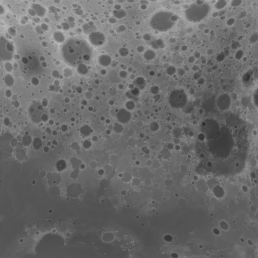
\includegraphics[width=0.24\textwidth]{fig/dtmh2.png}
  
\includegraphics[width=0.24\textwidth]{fig/blank.pdf}
  
\includegraphics[width=0.24\textwidth]{fig/blank.pdf}\\\vspace{1pt}
  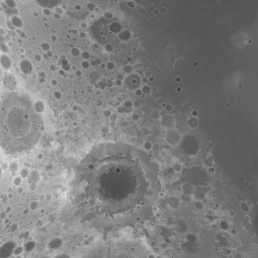
\includegraphics[width=0.24\textwidth]{fig/dtmh1.png}
  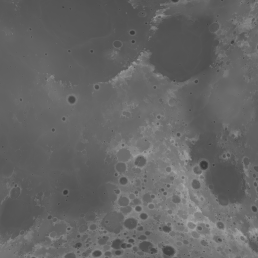
\includegraphics[width=0.24\textwidth]{fig/dtmh4.png}
  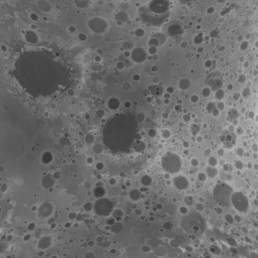
\includegraphics[width=0.24\textwidth]{fig/dtmh0.png}
  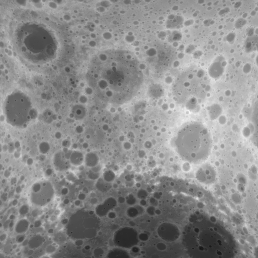
\includegraphics[width=0.24\textwidth]{fig/dtmh5.png}\\\vspace{1pt}
  
\includegraphics[width=0.24\textwidth]{fig/blank.pdf}
  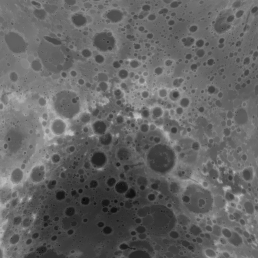
\includegraphics[width=0.24\textwidth]{fig/dtmh3.png}
  
\includegraphics[width=0.24\textwidth]{fig/blank.pdf}
  
\includegraphics[width=0.24\textwidth]{fig/blank.pdf}
  \caption{The six root pages of the lunar height map \scm.}
  \label{fig:dtmh}
\end{figure}

\subsection{A Normal Map}
\label{sec:normal}

The height map generated in the previous section enables a great many visualization tasks and modes, but the highest-quality real-time illumination of it requires the derivation of a normal map. A normal map gives a surface vector for each height map sample. To compute these vectors, both the radius of the sphere and the normalization of the height must be known.

The moon has an average radius of \SI{1737400}{\meter}. \texttt{DTM.tif} was prepared using a normalization of $(\num{-9160},\num{10770})$. Thus, the interpretation of \texttt{DTM.tif} is that a value of $0$ maps onto the radius $r_0=\SI{1737400}{\meter}-\SI{9160}{\meter}=\SI{1728240}{\meter}$ and a value of $1$ (represented in the 16-bit unsigned \tiff\ by \texttt{0xFFFF}) maps onto $r_1=\SI{1737400}{\meter}+\SI{10770}{\meter}=\SI{1748170}{\meter}$. These are the values to provide to the \texttt{normal} process.

\begin{Verbatim}
scmtiff -p normal -o DTM-O.tif -R 1728240,1748170 DTM.tif
\end{Verbatim}

The output of the normal process is neither bordered nor finished, so it is written to a temporary file. By convention, an unbordered normal map has the suffix \texttt{O}. Bordering and finishing produce the usable normal map, given the suffix \texttt{N}.

\begin{Verbatim}
scmtiff -p border -o DTM-N.tif DTM-O.tif
scmtiff -p finish DTM-N.tif
\end{Verbatim}

The six root faces of this \scm\ are shown in Figure~\ref{fig:dtmn}. In normal maps, positive $X$-facing surfaces appear red, positive $Y$ appears green, positive $Z$ appears blue.

\begin{figure}
  \centering
  
\includegraphics[width=0.24\textwidth]{fig/blank.pdf}
  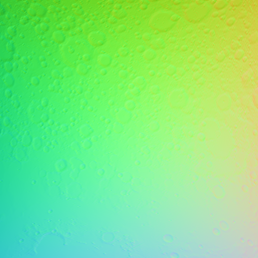
\includegraphics[width=0.24\textwidth]{fig/dtmn2.png}
  
\includegraphics[width=0.24\textwidth]{fig/blank.pdf}
  \includegraphics[width=0.24\textwidth]{fig/blank.pdf}\\\vspace{1pt}
  \includegraphics[width=0.24\textwidth]{fig/dtmn1.png}
  \includegraphics[width=0.24\textwidth]{fig/dtmn4.png}
  \includegraphics[width=0.24\textwidth]{fig/dtmn0.png}
  \includegraphics[width=0.24\textwidth]{fig/dtmn5.png}\\\vspace{1pt}
  \includegraphics[width=0.24\textwidth]{fig/blank.pdf}
  \includegraphics[width=0.24\textwidth]{fig/dtmn3.png}
  \includegraphics[width=0.24\textwidth]{fig/blank.pdf}
  \includegraphics[width=0.24\textwidth]{fig/blank.pdf}
  \caption{The six root pages of the lunar normal map \scm.}
  \label{fig:dtmn}
\end{figure}

\section{Automation}
\label{sec:automation}

For input images larger than a gigapixel or two, the \scm\ conversion process will take time. Because this is a multi-step process, it is convenient to automate it and allow it to run in a batch-oriented mode. The most basic way to do so is to write a shell script that issues each of the above command lines in turn. This approach can be modularized using shell variables and loops, and works well in simple cases. However, a more sophisticated approach uses the \texttt{make} utility to define the relationships between the inputs and outputs of each step of the conversion and adaptively determine the necessary order of operations automatically. The primary advantages to the use of \texttt{make} in this context are that it correctly handles interrupted conversion processes without expending redundant effort, and it intelligently exploits opportunities for process-level parallelism.

The following is an example \texttt{Makefile} that converts the equirectangular portion of the WAC GLD100 data set to a bordered, finished height map, and derives from this a bordered, finished normal map.

\begin{Verbatim}
N    = 426
D    = 6
NAME = GLD-$(N)-$(D)

TIFS =  WAC_GLD100_E300N0450_100M.tif \
        WAC_GLD100_E300N1350_100M.tif \
        WAC_GLD100_E300N2250_100M.tif \
        WAC_GLD100_E300N3150_100M.tif \
        WAC_GLD100_E300S0450_100M.tif \
        WAC_GLD100_E300S1350_100M.tif \
        WAC_GLD100_E300S2250_100M.tif \
        WAC_GLD100_E300S3150_100M.tif

all: $(NAME)-N.tif

%.tif: %.IMG
        scmtiff -p convert -n$(N) -d$(D) -N-9160,10770 -o $@ $<

$(NAME)-M.tif: $(TIFS)
        scmtiff -p combine -o $@ $<
        scmtiff -p mipmap $@

$(NAME).tif: $(NAME)-M.tif
        scmtiff -p border -o$@ $<
        scmtiff -p finish -t desc.txt $@

$(NAME)-O.tif: $(NAME).tif
        scmtiff -p normal -R1728240,1748170 -o$@ $<

$(NAME)-N.tif: $(NAME)-O.tif
        scmtiff -p border -o $@ $<
        scmtiff -p finish -t desc.txt $@
\end{Verbatim}

The variables \texttt{N} and \texttt{D} set the page size and tree depth (lines 1--2), which are carried throughout the process, making it easy to reprocess a single input at different resolutions. The variable \texttt{NAME} is defined in terms of these values (line 3), as per the \scm\ naming convention. Following this, the variable \texttt{TIFS} gives a list of constituent \scm\ \tiff\ files generated by the initial conversion (lines 5--12).

The \texttt{Makefile} lists the \tiff s instead of the \img s to enable the magic that happens next, in the \texttt{convert} recipe (lines 16--17). This is an abstract definition of the process of converting an \img\ to a \tiff, including its \scm\ parameters, description, and normalization. When \texttt{make} is informed by the \texttt{combine} recipe that these \tiff s are required, it knows how to convert them from \img s.

The \texttt{combine} recipe (lines 19--21) produces a single output given the eight inputs, and automatically executes the \texttt{mipmap} process on it in-place. By convention, this combined, mipmapped output is identified by the suffix \texttt{M}.

The \texttt{border} recipe (lines 23--25) re-encodes this \texttt{M} file with bordered pages, and finishes it, giving the height map output \texttt{GLD-426-6.tif}.

The \texttt{normal} recipes (lines 27--32) convert the finished height map to an intermediate normal map with the suffix \texttt{O}, which is bordered and finished giving a normal map \texttt{GLD-426-6-N.tif}.

In all cases, an output is defined in terms of its input and is annotated with the process necessary to perform the conversion. The build is invoked with a single command.

\begin{Verbatim}
make
\end{Verbatim}

This command considers all recipes, compares each output with its required input, and determines the minimum number of steps necessary to produce the output. Being aware of all dependencies, it will optionally execute non-interfering processes in parallel. To allow up to four simultaneous \img\ conversions,

\begin{Verbatim}
make -j4
\end{Verbatim}

This \texttt{Makefile} example is simplified from the complete planetary dataset example of Section~\ref{sec:planet}. It glosses over issues of blending and combining. A full \texttt{Makefile} capable of performing the complete lunar map conversion is given in Appendix~\ref{cha:makefile}.

%------------------------------------------------------------------------------

\chapter{\scm\ Render Library}

The \scm\ renderer is implemented as a small C++ library that may be embedded within any \opengl\ host application.

\section{\api}
\label{sec:api}

The \api\ provides three primary classes: a \emph{cache} class that manages \scm\ data and implements demand-paging with a least-recently-used ejection policy, a \emph{model} class that renders adaptive spherical geometry to which the cached imagery is applied, and a \emph{label} class that optionally annotates the sphere and its imagery. An application that renders \scm\ data will require at least one cache object and one model object.

The document lists the \emph{application} \api\ for each class, and includes only those methods of use to rendering applications. These classes do have other public methods, though they are generally reserved for intercommunication.

\bigskip\noindent\textit{class scm\_cache} has the following public methods.

\begin{itemize}
  \item\textit{scm\_cache(int size)}

    Construct a new cache object with the given maximum cache size (in pages).

  \item \textit{int add\_file(const std::string\& scm)}

    Add the named \scm\ \tiff\ file to the cache an integer descriptor for that file. A cache supports an arbitrary number of simultaneous files, and an application will usually have exactly one cache object per \opengl\ context.

  \item\textit{void update(int time)}

    Update the state of the cache using the given time value. To keep a cache and model in sync, and to properly manage page aging, this argument should given the value returned by \textit{sph\_model::tick}.

  \item\textit{void draw()}

    Draw the entire contents of the cache in thumbnail to a \twod\ on-screen rectangle.

\end{itemize}

\noindent\textit{class scm\_model} has the following public methods.

\begin{itemize}
  \item\textit{scm\_model(scm\_cache\& cache, const std::string\& vert,\\
      \phantom{scm\_model(scm\_cache\& cache,} const std::string\& frag,\\
      \phantom{scm\_model(scm\_cache\& cache,} int mesh, double r0, double r1)}

      Construct a new adaptive spherical model that renders \scm\ data in \textit{cache} using the vertex and fragment shaders \textit{vert} and \textit{frag}. The tessellation density is given by \textit{mesh} and the maximum expected range of displaced radii are \textit{r0} and \textit{r1}.

  \item\textit{int tick()}

    Advance and return the current model time. This value is passed to \textit{scm\_cache::update} and helps manage page age and latent-data fade-in.

  \item\textit{void prep(const double *P, const double *V, int w, int h)}

    Pre-process the model for rendering to a $w\times h$ buffer. \textit{P} gives the current $4\times 4$ projection matrix and \textit{V} gives the $4\times 4$ model-view matrix. This function iterates over the \scm\ hierarchy and determines which pages are in view (given these transformations) and at what resolution they appear (given this buffer size).

  \item\textit{void draw(const double *P, const double *V, const int *vv, int vc,\\
      \phantom{void draw(const double *P, const double *V,} const int *fv, int fc,\\
      \phantom{void draw(const double *P, const double *V,} const int *pv, int pc)}

    Draw the model using projection matrix \textit{P} and model-view matrix \textit{V}. The arrays \textit{vv}, \textit{fv}, and \textit{pv} give file descriptors (as returned by \textit{scm\_cache::add\_file}) to be supplied to the vertex shader, the fragment shader, and the pre-loader, respectively. The values \textit{vc}, \textit{fc}, and \textit{pc} give the length of each of these arrays.

\end{itemize}

\section{\scm\ path}
\label{sec:scmpath}

This library has just one system-level configuration parameter:

\scmpath\ is a shell environment variable akin to the bash executable path. It lists directories where \scm\ \tiff\ files may be found. If the application requests that the renderer load a file, but the renderer cannot find that file, then it will search this list of directories. Set this variable in the shell resource file, as need be, separated by colons. For example,

\begin{Verbatim}
export SCMPATH=/share/scm:$HOME/data/scm:.
\end{Verbatim}

For cluster-driven display systems, try to replicate all \scm\ \tiff s to local directories on all rendering nodes. This will perform better than data files stored on network shares.

\begin{table}
  \begin{tabular*}{\textwidth}{rcl}\hline
    \texttt{scm-basic.vert}    & \ldots & For static spheres. \T\\
    \texttt{scm-zoom.vert}     & \ldots & For zoomable panoramic \scm s. \\
    \texttt{scm-displace.vert} & \ldots & Displacement-mapped planetary \scm s. \B\\\hline
  \end{tabular*}
  \caption{\scm\ viewer vertex shaders}
  \label{tab:vert}
\end{table}

\begin{table}
  \begin{tabular*}{\textwidth}{rcl}\hline
    \texttt{scm-basic.frag}    & \ldots & Basic application of \scm\ color.\T\\
    \texttt{scm-blend.vert}    & \ldots & Blending and animation of \scm\ sequences.\\
    \texttt{scm-colormap.vert} & \ldots & False color mapping of single-channel \scm s.\\
    \texttt{scm-lomsee.vert}   & \ldots & Lommel-Seeliger shading with color and normal.\B\\\hline
  \end{tabular*}
  \caption{\scm\ viewer fragment shaders}
  \label{tab:frag}
\end{table}

%------------------------------------------------------------------------------

\chapter{\scm\ Example Applications}

Two example \scm\ rendering applications have been implemented using the Thumb framework, which enables cross-platform portability and scalability from laptops to cluster-driven virtual reality environments. The first of these applications, \panoview, renders \scm files inside-out and is suitable for high-resolution spherical panorama rendering. The second, \orbiter, renders \scm\ files outside-in and is suitable for planetary rendering. While the previous chapter on \scm\ handling applies to any embedding of the \scm\ renderer, this chapter specifically describes the configuration and usage of \panoview\ and \orbiter.

\section{Sphere Definition File}
\label{sec:scmxml}

The sphere definition is an \xml\ file that organizes \scm\ images into visualization and gathers all of the information required by the renderer.

As Thumb-based applications, \panoview\ and \orbiter\ must be able to find these \xml\ files. They appear in the Thumb data hierarchy like any other configuration file. This means they may be placed in a data directory rooted at the current directory, or in the \texttt{\textasciitilde/.thumb} hierarchy, or in a data hierarchy given by the \verb|THUMB_RO_PATH| environment variable. Sphere definition files need not be stored along side the \scm\ \tiff\ files that they reference, as the \scmpath\ environment variable still defines the location of \scm\ \tiff s.

\subsection{Basic Stereo Panorama}

Here is \texttt{Bluebonnet-0.xml}, a basic stereoscopic panorama definition.

\begin{Verbatim}
<?xml version="1.0"?>
  <sphere vert="glsl/scm-zoom.vert"
          frag="glsl/scm-basic.frag"
          mesh="16" radius="6">
    <scm channel="0" file="Bluebonnet-0-L-512-4.tif" />
    <scm channel="1" file="Bluebonnet-0-R-512-4.tif" />
  </sphere>
\end{Verbatim}

The file begins with an \xml\ header and contains a single root sphere element with optional attributes and one sub-element for each \scm\ image.

The \texttt{vert} and \texttt{frag} attributes (lines 2--3) give the vertex and fragment shaders to be used by the renderer, named relative to the root of the Thumb data hierarchy. Tables~\ref{tab:vert} and~\ref{tab:frag} list the available shaders. This example is a single high-resolution stereoscopic panorama. It should be zoomable, yet it requires no special pixel processing, so the \texttt{scm-zoom.vert} vertex shader and the \texttt{scm-basic.frag} fragment shader are specified.

The \texttt{mesh} attribute (line 4) of the sphere element determines the tessellation density of the geometry mesh used to render each page of data. The example value, 16, indicates that each page of the sphere will be rendered using a $16\times 16$ grid of polygons. This is the default, and is an appropriate value for panoramas.

The \texttt{radius} attribute (line 4) determines the radius of the spherical geometry to which the \scm\ imagery is applied. This value is given in meters, and is most significant in determining the apparent scale of the sphere in a VR display environment.

The \texttt{scm} sub-elements (lines 5--6) give the \scm\ file names. The \texttt{channel} attributes indicate which stereoscopic channel each \scm\ provides.

\subsection{Multi-image Panorama}

This example, \texttt{Taliesin-Path.xml}, is a more complex stereoscopic panorama giving a series of images for each channel. The \texttt{scm} elements are wrapped in \texttt{frame} groups and organized into a sequence. The \texttt{frag} attribute of the \texttt{sphere} element specifies the \texttt{scm-blend.frag} fragment shader, which fades smoothly from one frame to the next. The result is a panoramic virtual reality walk down a garden path at Taliesin.

\begin{Verbatim}
<?xml version="1.0"?>
  <sphere vert="glsl/sph-zoomer.vert"
          frag="glsl/sph-blend.frag">
    <frame>
      <scm channel="0" file="Taliesin-Path-A-L-512-3.tif" />
      <scm channel="1" file="Taliesin-Path-A-R-512-3.tif" />
    </frame>
    <frame>
      <scm channel="0" file="Taliesin-Path-B-L-512-3.tif" />
      <scm channel="1" file="Taliesin-Path-B-R-512-3.tif" />
    </frame>
    <frame>
      <scm channel="0" file="Taliesin-Path-C-L-512-3.tif" />
      <scm channel="1" file="Taliesin-Path-C-R-512-3.tif" />
    </frame>
    <frame>
      <scm channel="0" file="Taliesin-Path-D-L-512-3.tif" />
      <scm channel="1" file="Taliesin-Path-D-R-512-3.tif" />
    </frame>
    <frame>
      <scm channel="0" file="Taliesin-Path-E-L-512-3.tif" />
      <scm channel="1" file="Taliesin-Path-E-R-512-3.tif" />
    </frame>
    <frame>
      <scm channel="0" file="Taliesin-Path-F-L-512-3.tif" />
      <scm channel="1" file="Taliesin-Path-F-R-512-3.tif" />
    </frame>
    <frame>
      <scm channel="0" file="Taliesin-Path-G-L-512-3.tif" />
      <scm channel="1" file="Taliesin-Path-G-R-512-3.tif" />
    </frame>
    <frame>
      <scm channel="0" file="Taliesin-Path-H-L-512-3.tif" />
      <scm channel="1" file="Taliesin-Path-H-R-512-3.tif" />
    </frame>
  </sphere>
\end{Verbatim}

\subsection{Displacement-mapped Illuminated Planet}

The following example brings together multiple disparate data sets to produce a displacement-mapped sphere with real-time illumination and diffuse color, suitable for viewing with \texttt{orbiter}. It demonstrates a number of additional attributes.

\begin{Verbatim}
<?xml version="1.0"?>
  <sphere mesh="128" r0="0.994728" r1="1.0062" radius="20.0"
            vert="glsl/scm-displace.vert"
            frag="glsl/scm-lomsee.frag">
    <scm shader="vert" file="DTM-426-6.tif" />
    <scm shader="frag" file="DTM-426-6-N.tif" />
    <scm shader="frag" file="clementine-512-3.tif" />
  </sphere>
\end{Verbatim}

The \texttt{mesh} resolution has been increased to 128 from its default 16. This is because a height map \scm\ is applied to the sphere geometry by the \texttt{scm-displace.vert} vertex shader. The geometry must have a dense tessellation to allow a close mapping from height map samples to \threed\ vertices. Related to this, the \texttt{r0} and \texttt{r1} attributes give the magnitude of the displacement applied to that geometry, relative to a radius of $1$. These are the same values used when generating the normal map in Section~\ref{sec:normal}. $\texttt{r0}=\num{1728240} / \num{1737300}$ and $\texttt{r1}=\num{1748170} / \num{1737400}$.

The \texttt{scm} elements have an additional attribute, \texttt{shader}, which allows an \scm\ to be targeted toward a specific shader. In this case, the \texttt{scm-displace.vert} shader is granted access to the height map. The default shader target for \texttt{scm} elements is ``frag,'' which is given explicitly here for symmetry. This rendering uses the \texttt{scm-lomsee.frag} fragment shader which requires \emph{two} images, separately applied to the per-fragment normal and diffuse color coefficients of the Lommel-Seeliger lighting model. Order matters here, and this shader expects the normal map to be listed first.

It's worth noting that not all of the data sets used in this visualization have the same page size and depth. Equality in not required, and the adaptive renderer will defer to the lowest page size to ensure that an appropriate level of detail is achieved for all data. Likewise, the deepest \scm\ depth \emph{will} be fully utilized, and shallower \scm s will undergo linear magnification filtering to match.

\section{Panoview Usage}

\panoview\ and \orbiter\ are configured and run like any other Thumb application. The following keyboard commands are defined.

\begin{itemize}
\item[F1] Toggle the sphere definition file selection dialog. This dialog allows the user to navigate the Thumb data hierarchy and select a visualization definition for viewing.

\item[F2] Toggle the cache visualization overlay. This allows the set of all resident pages to be viewed in thumbnail.

\item[F3] Toggle the model label, if any.

\item[F4] Toggle the wire-frame view of the sphere geometry.

\end{itemize}

In addition, there is one option in the Thumb configuration file \texttt{conf.xml} that impacts the behavior and performance of these applications:

\begin{Verbatim}
<option name="scm_cache_size">128</option>
\end{Verbatim}

This option gives the value passed to the \texttt{scm\_cache} constructor, selecting the maximum number of pages that may be loaded at any given moment. A $512\times 512$ page of \rgb\ data consumes 1\mb\ of \vram\, and this cache size option should be set accordingly. A larger value gives better performance, but too large a value will result in catastrophically bad performance. Knowledge of your hardare's available \vram\ will help to determine the optimal value.

\section{Troubleshooting}

This is a list of issues to be aware of, should trouble arise when configuring or using \panoview\ and \orbiter.

\begin{itemize}
\item If the panorama definition \xml\ files are not visible in the sphere definition file selector, then be sure they are located within the Thumb data hierarchy, or add their location to the Thumb data hierarchy by including the path in the \verb|THUMB_RO_PATH| environment variable.

\item If the panorama definition loads but does not display an image, be sure the path to the \scm\ \tiff\ files appears in the \scmpath\ environment variable.

\item If a multi-image panorama jumps from one panorama to the next instead of fading, be sure the blend fragment program is referenced by the definition.

\item If performance is sluggish, be sure that panorama image files are not being accessed from a network share, and that the \texttt{conf.xml} setting of \verb|scm_cache_size| is not too high.
\end{itemize}


%-------------------------------------------------------------------------------

\appendix
\chapter{Integer Binary Logarithm}
\label{cha:log}

The following C Language function computes the 64-bit integer binary logarithm in $O(\log n)$ operations. It takes and returns a signed value, instead of unsigned, as this is the most appropriate C type for \scm\ page indices.

\begin{Verbatim}
static inline long long log2i(long long n)
{
    unsigned long long v = (unsigned long long) n;
    unsigned long long r;
    unsigned long long s;

    r = (v > 0xFFFFFFFFULL) << 5; v >>= r;
    s = (v > 0xFFFFULL    ) << 4; v >>= s; r |= s;
    s = (v > 0xFFULL      ) << 3; v >>= s; r |= s;
    s = (v > 0xFULL       ) << 2; v >>= s; r |= s;
    s = (v > 0x3ULL       ) << 1; v >>= s; r |= s;

    return (long long) (r | (v >> 1));
}
\end{Verbatim}

%-------------------------------------------------------------------------------

\chapter{LRO DTM Makefile}
\label{cha:makefile}

\begin{Verbatim}
N=426
D=6

NAME = DTM-$(N)-$(D)
FORM = -n $(N) -d $(D)
NORM = -N -9160,10770 -g 0
RADI = -R 1728240,1748170
TEXT = -t desc.txt

GLDE =\
        WAC_GLD100_E300N0450_100M.tif \
        WAC_GLD100_E300N1350_100M.tif \
        WAC_GLD100_E300N2250_100M.tif \
        WAC_GLD100_E300N3150_100M.tif \
        WAC_GLD100_E300S0450_100M.tif \
        WAC_GLD100_E300S1350_100M.tif \
        WAC_GLD100_E300S2250_100M.tif \
        WAC_GLD100_E300S3150_100M.tif
GLDP =\
        WAC_GLD100_P900N0000_100M.tif \
        WAC_GLD100_P900S0000_100M.tif
LOLA =\
        ldem_45n_100m.tif \
        ldem_45s_100m.tif

# Convert a raw normal map to a bordered and finished normal map.

$(NAME)-N.tif: $(NAME)-O.tif
        scmtiff -T -p border -o $@ $<
        scmtiff -T -p finish $(TEXT) $@

# Convert a height map into a raw normal map.

$(NAME)-O.tif: $(NAME).tif
        scmtiff -T -p normal $(RADI) -o $@ $<

# Border and finish.

$(NAME).tif: $(NAME)-M.tif
        scmtiff -T -p border -o $@ $<
        scmtiff -T -p finish $(TEXT) $@

# Combine the two projections and mipmap the result.

$(NAME)-M.tif: $(NAME)-E.tif $(NAME)-P.tif
        scmtiff -T -p combine -m avg -o $@ $^
        scmtiff -T -p mipmap $@

# Sum the equirectangular projections.

$(NAME)-E.tif: $(GLDE)
        scmtiff -T -p combine -m max -o $@ $^

# Sum the polar projections.

$(NAME)-P.tif: $(GLDP) $(LOLA)
        scmtiff -T -p combine -o $@ $^

# Convert all PDS files to TIFF.

WAC_GLD100_E%.tif: WAC_GLD100_E%.IMG
        scmtiff -T -p convert $(FORM) $(NORM) -o $@ $<

WAC_GLD100_P900N0000_100M.tif: WAC_GLD100_P900N0000_100M.IMG
        scmtiff -T -p convert $(FORM) $(NORM) -o $@ -P  90,12,11 $<

WAC_GLD100_P900S0000_100M.tif: WAC_GLD100_P900S0000_100M.IMG
        scmtiff -T -p convert $(FORM) $(NORM) -o $@ -P -90,12,11 $<

ldem_45n_100m.tif: ldem_45n_100m.lbl
        scmtiff -T -p convert $(FORM) $(NORM) -o $@ -P  90,11,12 $<

ldem_45s_100m.tif: ldem_45s_100m.lbl
        scmtiff -T -p convert $(FORM) $(NORM) -o $@ -P -90,11,12 $<

clean:
        rm -f $(NAME).tif $(GLDE) $(GLDP) $(LOLA)
\end{Verbatim}

\printpagenotes
\end{Spacing}
\end{document}
